\documentclass[11pt]{report}

% the recommended packages discussed in section 4. Keep them!
\usepackage{pkgs/rtsched}
\usepackage[sorting=none]{biblatex}
\usepackage{parskip}
\usepackage{booktabs}
\usepackage{siunitx}
\sisetup{per-mode=symbol} 
\usepackage{pgfgantt}
\usepackage{rotating}
\usepackage{vhistory}
\usepackage{pgfplots}
% \usepgfplotslibrary{external}
% \tikzexternalize
\usepackage{pgfplotstable}
\usepackage{tikz}
\usepackage{caption}
\usepackage{subcaption}
\usepackage{adjustbox}
\usepackage{eqexpl}
\eqexplSetIntro{where:} % set parenthesis in the left of the first item
\eqexplSetDelim{=} % set delimiter to "="
\usepackage{bytefield}
\usepackage{xcolor}
\usepackage{amsfonts}
\usepackage{amsmath}
\usepackage{graphicx}
\usepackage{wheelchart}
\usepackage{etoolbox}
\usepackage{listofitems}
\usetikzlibrary{decorations.text}
\usepackage{lipsum}
\usepackage{import}
\usepackage[colorinlistoftodos]{todonotes}
\usepackage{pgf-pie}  
\usepackage{multirow}
\usepackage{threeparttable}

\definecolor{lightcyan}{rgb}{0.84,1,1}
\definecolor{lightgreen}{rgb}{0.64,1,0.71}
\definecolor{lightred}{rgb}{1,0.7,0.71}
\definecolor{lightorange}{rgb}{1,0.8,0.5}
\definecolor{lightpurple}{rgb}{0.89,0.79,0.96}
\definecolor{lightyellow}{rgb}{0.92,0.99,0.48}
\definecolor{lightgray}{gray}{0.8}

% \definecolor{blue}{rgb}{0,0,1}
\definecolor{bluehue1}{RGB}{0, 76, 109}
\definecolor{bluehue2}{RGB}{17, 109, 141}
\definecolor{bluehue3}{RGB}{38, 143, 173}
\definecolor{bluehue4}{RGB}{63, 180, 202}
\definecolor{bluehue5}{RGB}{92, 217, 230}
\definecolor{bluehue6}{RGB}{126, 255, 255}

% some packages required for typesetting a nice manual
\usepackage{tabularx}
\usepackage[a4paper]{geometry}
\usepackage{listings}
\lstset{language=tex, frame=single, basicstyle=\small}
\usepackage{shortvrb}
\MakeShortVerb{\|}
\usepackage{titlesec}
\newcommand{\sectionbreak}{\clearpage}

% load the titlepage providing package. Mind the slash!
\usepackage[affiliation=double,corporate-identity=none]{tu/e}

% its good practice to always load the ~ref packages last, in this order:
\usepackage{hyperref}
\hypersetup{colorlinks=true,urlcolor=blue,linkcolor=blue,citecolor=red}
\usepackage[nameinlink]{cleveref}

\DeclareMathOperator{\eread}{E_{\textrm{read}}}
\DeclareMathOperator{\ereadlpddr5x}{E_{\textrm{read,LPDDR5X}}}
\DeclareMathOperator{\ereadpcm}{E_{\textrm{read,PCM}}}
\DeclareMathOperator{\ephy}{E_{\textrm{phy}}}
\DeclareMathOperator{\ectrl}{E_{\textrm{ctrl}}}
\DeclareMathOperator{\eaxi}{E_{\textrm{axi}}}
\DeclareMathOperator{\enoc}{E_{\textrm{noc}}}
\DeclareMathOperator{\ewrite}{E_{\textrm{write}}}
\DeclareMathOperator{\econf}{E_{\textrm{conf}}}
\DeclareMathOperator{\econflpddr5x}{E_{\textrm{conf,LPDDR5X}}}
\DeclareMathOperator{\econfpcm}{E_{\textrm{conf,PCM}}}
\DeclareMathOperator{\eproc}{E_{\textrm{proc}}}

\DeclareMathOperator{\lattotal}{lat_{total}}
\DeclareMathOperator{\latconf}{lat_{conf}}
\DeclareMathOperator{\latproc}{lat_{proc}}
\DeclareMathOperator{\size}{size}
\DeclareMathOperator{\mappable}{mappable}
% \DeclareMathOperator{\econf}{E_{conf}}
% \DeclareMathOperator{\eproc}{E_{proc}}
\DeclareMathOperator{\etotal}{E_{total}}
\DeclareMathOperator{\eddrread}{E_{ddr\_read}}
\DeclareMathOperator{\eddrphy}{E_{ddr\_phy}}
\DeclareMathOperator{\eddrctrl}{E_{ddr\_ctrl}}
% \DeclareMathOperator{\eaxi}{E_{axi}}
% \DeclareMathOperator{\enoc}{E_{noc}}
\DeclareMathOperator{\esramwrite}{E_{sram\_write}}
\DeclareMathOperator{\readamount}{R}
\DeclareMathOperator{\writeamount}{W}
\DeclareMathOperator{\coresused}{C}
\DeclareMathOperator{\avgutil}{U}
\DeclareMathOperator{\writebandwidth}{BW_{\textrm{write}}}
\DeclareMathOperator{\pcore}{P_\textrm{core}}

\DeclareMathOperator{\eextmem}{E_\textrm{ext\_mem}}
\DeclareMathOperator{\ereadextmem}{E_\textrm{read\_ext\_mem}}
\DeclareMathOperator{\esendtonoc}{E_\textrm{send\_to\_noc}}
\DeclareMathOperator{\nhops}{N_\textrm{hops}}
\DeclareMathOperator{\ehop}{E_\textrm{hop}}
\DeclareMathOperator{\ptotal}{p_\textrm{total}}
\DeclareMathOperator{\pdata}{p_\textrm{data}}

\DeclareMathOperator{\relu}{ReLU}

\newcommand{\snap}{Snap Inc.}
\newcommand{\graicore}{GrAICore}
% \newcommand{\graipefruit}{GrAIPEFRUIT}
\newcommand{\confignoc}{Config NoC}
\newcommand{\eventnoc}{Event NoC}



% Use these macros to supply information for on your titlepage. The must be
% placed in the preamble! You can safely omit any of them if you don't want to
% print that specific bit of information to the titlepage.
\title{Exploring efficient reconfiguration on the GrAICore}
% \subtitle{Hello world}
\thesistype{Master thesis}
\idnumber{1712918}
\author{S. Yip}
\supervisors{Supervisors\\dr.ir. M.C.W. Geilen (TU/e)\\dr. Hamid Tabani (Snap Inc.)\\dr.ir. Orlando Moreira (Snap Inc.)}
\version{Draft version}
\citydate{Eindhoven, November 2024}
\institutioninfo{Department of Electrical Engineering\\Electronic Systems Group}
\secondinstitutionlogo[height=2cm]{assets/snap_logo.png}
\secondinstitutioninfo{Snap Inc.\\Snap Lab Hardware Engineering}

\addbibresource{references.bib}

% \linespread{1.5}
\begin{document}
\onehalfspacing

\begin{versionhistory}
  \vhEntry{0.1}{September 30, 2024}{S. Yip}{Initial draft}
  \vhEntry{0.2}{October 22, 2024}{S. Yip}{Second draft}
\end{versionhistory}
\chapter*{Abstract}
\lipsum[1]


\tableofcontents

\chapter{Introduction}
\import{sections/introduction}{problem_statement}
\import{sections/introduction}{research_question}
\import{sections/introduction}{outline}

\chapter{Background}
\import{sections/background}{edge_ai}
\import{sections/background}{computer_vision}
\import{sections/background}{neural_networks}
\import{sections/background}{ai_accelerator}
\import{sections/background}{noc}
\import{sections/background}{external_memory}
\import{sections/background}{graicore}
% \import{sections/background}{swapping}

\chapter{Evaluation of the config NoC}
\import{sections}{config_noc_eval}

\chapter{Model execution analysis}
\import{sections/model_execution_analysis}{multi_model}
\import{sections/model_execution_analysis}{large_model}

\chapter{Config NoC bandwidth improvements}
\import{sections/bandwidth_improvements}{bandwidth_improvements}
\import{sections/bandwidth_improvements}{proposed_changes}

\chapter{Power analysis} \label{chapter:power_analysis}
\import{sections}{power_analysis}

\chapter{Model configuration improvements} \label{chapter:model_configuration_improvements}
\import{sections}{model_configuration_improvements}
\import{sections/model_configuration_improvements}{states}
\import{sections/model_configuration_improvements}{weight_duplications}
\import{sections/model_configuration_improvements}{pruning}
% \import{sections/model_configuration_improvements}{quantization}
\import{sections/model_configuration_improvements}{conclusion}

% \chapter{Exploring partitioning strategies}

\chapter{Partitioning large models - Formal problem description}
% \section{Large model partitioning}
\label{section:tmp}
\lipsum[1]

\chapter{Conclusion}
\lipsum[1]

\chapter{Future work}
\section{Exploring partitioning strategies}
\import{sections}{exploring_partitioning}
\section{Parallel configuration/processing}
Explain that we can speed up inference of large models by configuring and processing the partitions in parallel or pipelined.

\section{Compiler analysis}
Explain that with a comprehensive analysis of the compiler, we can improve the search for optimal solutions for a model or model partition.

\section{Add static power consumption}
Explain that we have only considered dynamic power/energy consumption.
Static power has not been explored.

\section{Other memory technologies}
We have only explored two specific memory technologies (DDR).
Using an other memory technology may provide us with better results.
This could be in terms of speed and energy use.

The energy numbers of PCM looks more promising compared to the LPDDR5X memory.
However, a few parameters haven't been considered in this research.
For example, the density (capcity per physical area) of LPDDR5X is higher than PCM.

\section{}
% Recent trends in artificial intelligence (AI) development indicate a substantial surge in the complexity and size of AI models since the advent of the Deep Learning Era \cite{EpochDatabaseVisualization}.
Sophisticated state-of-the-art AI models, such as those used in natural language processing and image recognition, can vary widely in complexity, with some containing as few as thousands of parameters and others exceeding a trillion.
These parameters are the fundamental components that AI models manipulate to learn from data and make predictions or decisions.
Processing such huge models requires an extensive amount of computational power.
High-performance computing systems with powerful GPUs and large memory pools are typically employed to train these models as well as to perform inference using them.
However, the deployment of AI solutions is not limited to these high-resource environments.
There is a significant push to bring AI capabilities closer to the end-users, which is where edge computing comes into play.
This shift is primarily motivated by the need for reduced latency, ensuring that decisions and actions can be taken almost instantaneously, and by the importance of low power consumption.



% \section{Problem statement}

The problem to be addressed by this project is the inability to reconfigure the GrAICore during run-time.
The current design of the GrAICore is incapable of doing this due to the limited host to GrAICore interface.
Adding this feature for the GrAICore to reconfigure during run-time significantly enhances its capabilities.
Firstly, it will allow multiple computer vision models to be used simultaneously while the GrAICore is running.
Deploying multiple computer vision models can be highly beneficial for creating a multifaceted system capable of handling diverse tasks simultaneously.
Each model can be specialized for a specific function, allowing the system to be more versatile and responsive to different visual processing requirements.
Secondly, using a technique such as partitioning the neural network into parts, allows the GrAICore to manage large models that do not fit on the GrAICore at once.
This method processes one model part at a time, requiring only a part of the model to be loaded.
Larger computer vision models for inference typically offer higher accuracy and better generalization to new data, can capture more complex features, and are more robust to noise and distortions.
They are valuable for tasks requiring the utmost precision.

Additionally, as specified by GML, they require that the GrAICore supports seamless reconfiguration.
In this context, seamless reconfiguration refers to the ability to switch between different AI models, or to modify the current model, without interrupting or significantly delaying data processing.
Given that the GrAICore is focused on computer vision applications, this means that it is crucial that the processing of input images occurs in a timely manner.
This is particularly challenging for video applications, where each frame must be processed before the next one arrives. Failing to meet this requirement can reduce the usefulness of the results, thereby degrading the system's quality of service.
Specifically, GML requires the system to support an incoming video frame rate of \SI{60}{FPS}.

% \section{Research question}

Due to the limited local memory of the GrAICore, it can only support AI models of a certain size.
This limitation becomes a roadblock for scenarios where larger models are needed for improved accuracy or when multiple models need to be deployed simultaneously.
The introduction of external memory is a potential solution to this challenge, but it requires careful integration to maintain the energy efficient, high-speed and low-latency performance expected from edge devices.

Ultimately, this project aims to answer the following research question:

\textbf{How can the architectural design of the GrAICore be adapted to enable seamless reconfiguration?}

To address this overarching question, the project will explore several sub-research questions:

\begin{itemize}
    \item \textbf{Supporting multiple models:}
    \begin{itemize}
        \item What modifications are necessary to support switching between multiple AI models for videos up to \SI{60}{FPS}?
    \end{itemize}
    \item \textbf{Supporting large models:}
    \begin{itemize}
        \item What strategies can be employed to support the execution of large AI models?
    \end{itemize}
    \item \textbf{Sustainable power consumption:}
    \begin{itemize}
        \item How can sustainable power consumption be ensured while maintaining performance?
    \end{itemize}
\end{itemize}
% \section{Outline}

\lipsum[1]


% \chapter{Background}

\lipsum[1]

% \subsection{AI at the edge}
% \section{AI at the edge}

Edge devices are often the frontline for data collection and user interaction, making them crucial for applications that require real-time processing, such as facial recognition on smartphones or decision-making in autonomous vehicles.
These devices are characterized by their compact size and energy efficiency.
However, the compute capacities of edge devices are considerably lower than those of dedicated AI cloud servers.
This presents a significant challenge for deploying sophisticated AI models directly onto edge devices.
Given the constraints of memory and processing power on the edge, it is crucial to adapt models to operate within these limitations while striving to maximize their efficacy.

To bridge this gap, AI researchers and engineers have developed several model compression techniques \cite{neill_overview_2020}.
One such technique is quantization, which reduces the precision of a model's numerical parameters.
For example, instead of using 32-bit floating-point numbers, a model might use 16-bit or even 8-bit representations, which can drastically cut down the memory requirement and computational costs.
Another technique is pruning, which removes parameters that contribute little to the model's outputs.
This is like removing the least essential parts of a complex machine without affecting its overall functionality.
The challenge with pruning is to identify which parts of the model can be removed with the smallest impact on its performance.
These model optimization techniques are crucial for maintaining a balance between performance and efficiency.
They aim to minimize the impact on the model's accuracy and predictive capabilities while significantly reducing its memory footprint and computational requirements.

In addition, hardware innovations have emerged to bridge the gap between the computational demands of AI models and the capabilities of edge devices.
The emergence of edge AI accelerators is a clear indicator of this trend.
These specialized processors are engineered to perform the matrix operations and linear algebra that are fundamental to AI computations with high efficiency and low power consumption.
By integrating these accelerators into edge devices, it is possible to execute complex AI models more effectively within the stringent constraints of power, space, and computing resources typical of edge environments.

Although optimization techniques can reduce the memory and computational demands of AI models, the internal memory in edge AI accelerators is inherently limited due to their compact size and design constraints aimed at conserving energy and space.
This limitation can be a significant bottleneck, especially as AI models become more complex and require more data to function optimally.
Internal memory may not be sufficient to store large models or to handle multiple models running simultaneously, which is increasingly necessary for more advanced applications.

To overcome these limitations, there is a growing interest in exploring external memory solutions that can be integrated with edge AI accelerators.
External memory provides additional storage capacity and allows edge devices to support larger AI models or multiple models simultaneously without compromising performance.
Supporting large models on edge devices typically results in better accuracy compared to using smaller, compressed models. Additionally, running multiple models simultaneously allows for a wider array of functionalities.
Therefore, expanding the memory capacity through external solutions is an effective way to extend the potential of AI at the edge.

% \subsection{GrAICore}
% \section{GrAICore}

One of these edge AI accelerators is the GrAICore designed by GrAI Matter Labs (GML).
The GrAICore utilizes the ``NeuronFlow'' technology, a many-core architecture that is inspired by the neural structures of the brain \cite{moreiraNeuronFlowNeuromorphicProcessor2020}, \cite{moreira_neuronflow_2020}.
Its main use case is computer vision applications using models based on convolutional neural networks (CNNs).
It features a total of 144 neuron cores, arranged in a 12 by 12 grid.
A neuron core includes a local SRAM memory for storing data such as model parameters and a processing element for performing mathematical operations (see \cref{fig:neuron_core}).

\begin{figure}[htbp]
    \centering
    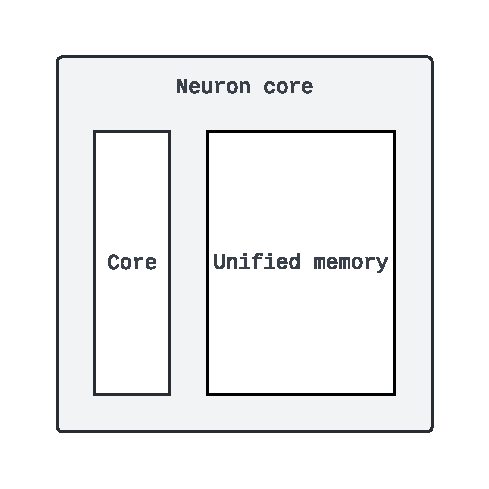
\includegraphics[width=0.25\textwidth]{assets/neuron_core.pdf}
    \caption{The neuron core includes a processing element (core) and a local memory (a.k.a. unified memory)}
    \label{fig:neuron_core}
\end{figure}

\subsubsection{Near-memory computing}
The GrAICore makes use of near-memory computing.
Near-memory computing refers to an computer architecture where computation is performed close to the memory.
This approach aims to mitigate the ``von Neumann bottleneck'', a limitation caused by the traditional computing architecture where the CPU (Central Processing Unit) and memory are separate entities, and data must be transferred back and forth between them \cite{indiveriMemoryInformationProcessing2015}.
By performing computations closer to where data is stored, data movement between the processing element and memory is minimized, reducing latency and energy consumption.
However, this introduces a constraint that requires the parameters of a model to reside in local memory before it can be used by the processing element.
Thus, an AI model must first be mapped and loaded onto the GrAICore before it can be used for inference.
Mapping means to assign the layers of a neural network to the neuron cores.
Intelligent mapping is important for balancing memory, computation and traffic between neuron cores.
The GrAICore features a total of \SI{36}{MB} of local memory, which is evenly distributed across its $144$ neuron cores.
The size of an AI model can be quantified by the number of its parameters.
For instance, if a parameter is stored as a 16-bit value on the GrAICore, it can accommodate approximately $\frac{\SI{36}{MiB}}{\SI{16}{b}}$ parameters\footnote{In practice, the available space for parameters is smaller because a portion of the memory is allocated for storing other relevant data.}, which translates to around \SI{19}{M} parameters in total.
Popular computer vision models like ResNet-50 \cite{heDeepResidualLearning2015} and YOLOv7 \cite{wangYOLOv7TrainableBagoffreebies2022}, with over \SI{25}{M} and \SI{37}{M} parameters respectively, are already too large by themselves to fit on the GrAICore.
Using optimization techniques, these models can be compressed into a smaller size.
For example, YOLOv7-tiny \cite{wangYOLOv7TrainableBagoffreebies2022} is a size optimized model of the YOLOv7 for edge devices at the cost of accuracy.
Its size is decreased to around \SI{6}{M} parameters, making it suitable for the GrAICore.
In summary, the number of parameters that can be stored on the GrAICore is limited by the size of its memory.
% Due to this, the GrAICore is only able to support limited sized AI models.

\begin{figure}[htbp]
    \centering
    \subfloat[The event NoC features a 2D torus topology]{
        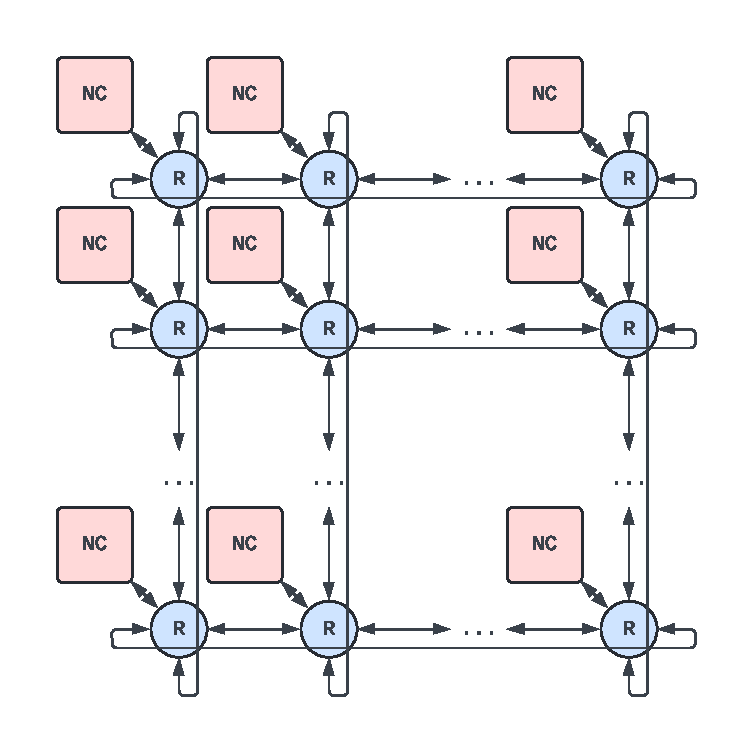
\includegraphics[width=0.45\textwidth]{assets/event_noc.pdf}
        \label{fig:event_noc}
    }
    \hfill
    \subfloat[The config NoC features a 2D mesh topology]{
        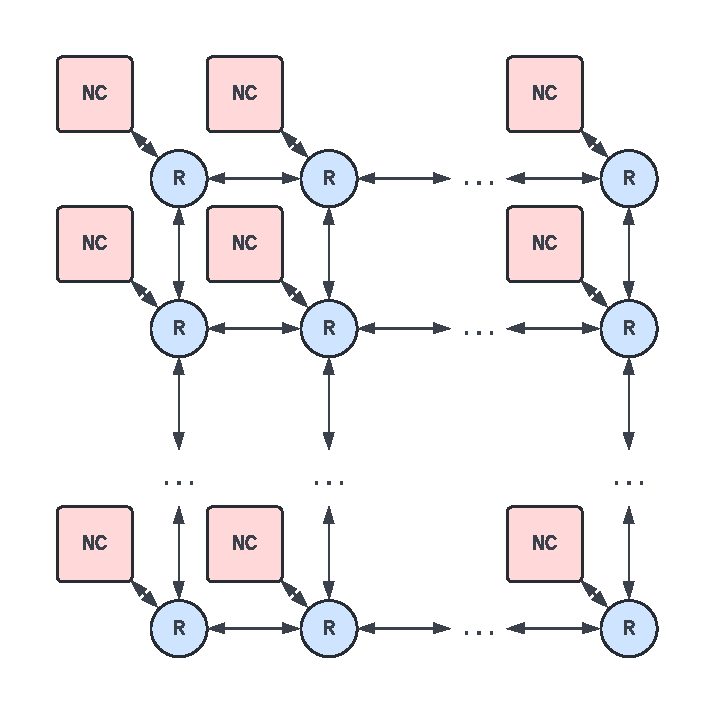
\includegraphics[width=0.45\textwidth]{assets/config_noc.pdf}
        \label{fig:config_noc}
    }
    \caption{GrAICore's network-on-chips. A neuron core (NC) communicates via its associated router (R) with other neuron cores and external parties such as the host device (not illustrated).}
    \label{fig:noc}
\end{figure}

\subsubsection{NoCs}
The neuron cores are connected to each other with two distinct network-on-chips (NoCs), each serving its own purpose (see \cref{fig:noc}).
% Firstly, the event NoC is responsible for transferring small packets of data called Events to its destination.
Firstly, the event NoC is used for exchanging activated neuron states in the form of small messages called Events.
Events are only generated when an AI model is being executed.
The event NoC uses the 2D torus topology.
Secondly, the config NoC is responsible for configuring the GrAICore, monitoring and debugging.
The config NoC uses a different topology, namely a 2D mesh topology.
Configuring the GrAICore means that the local memories of the neuron cores are written with the parameters of an AI model.
A host device (e.g., a microcontroller) initiates the configuration of the GrAICore.
The host device is connected to the config NoC via a single link, which is used to transfer data to and from any neuron core.
Since all data transfers must go through this link to reach its destination neuron core, it causes a significant bottleneck in data transfer speed to the GrAICore.
That is, the amount of data that can be transferred to the neuron cores within a certain time is poor as it was not designed with speed in mind.
Therefore, currently, the configuration of the memories of the neuron cores is only performed once at the start.
% This limitation restricts the GrAICore to be (partially) reconfigured at run-time.



% \subsection{Network-on-chip}
% \section{Network-on-chip}

Network-on-chip (NoC) has become a crucial component in modern multi-core systems-on-chip (SoCs), offering high throughput, low latency, and efficient power utilization.
The performance of NoCs is influenced by various factors such as topology, routing algorithms, switching mechanisms, and link/channel width.
In the quest for optimal performance, researchers have delved into exploring different aspects of NoC design to enhance its efficiency.
One key element that significantly impacts NoC performance is the choice of topology.
Studies have shown that selecting an appropriate topology is critical as it affects zero-load latency, sustainable bandwidth, and power consumption \cite{chenPhysicalVsVirtual2010}.
Studies have shown that selecting an appropriate topology is critical as it affects zero-load latency, sustainable bandwidth, and power consumption \cite{chen}.
For instance, the 2D mesh topology, as utilized in the GrAICore, is commonly used in NoCs due to its scalability and fault tolerance, enabling efficient communication among cores.

\begin{figure}[htbp]
\centering
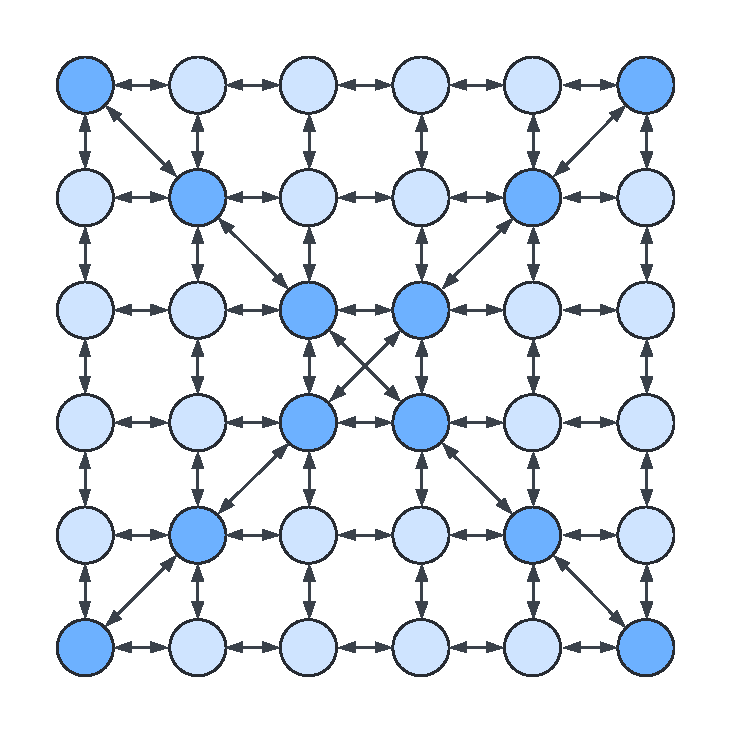
\includegraphics[width=0.45\textwidth]{assets/xdmesh_topology.pdf}
\caption{
An 6x6 XDMesh topology.
The darker blue shaded nodes feature additional diagonal links.
}
\label{fig:xdmesh_topology}
\end{figure}

Additionally, the extended diagonal mesh (XDMesh) has been proposed as an enhancement to the 2D mesh topology \cite{furhadExtendedDiagonalMesh2015}.
XDMesh improves the 2D mesh by incorporating diagonal links (see example in \cref{fig:xdmesh_topology}), which decrease the network diameter---the longest distance between two nodes situated at opposite diagonal corners of the 2D mesh.
This reduction in network diameter leads to lower communication delays and fewer  hop counts.
Experimental results show that XDMesh achieves over $40\%$ better throughput and latency compared to the 2D mesh.
Furthermore, it outperforms the 2D mesh in terms of energy efficiency, with minimal differences in silicon area.
The experimental environment makes use of the uniform traffic model, where each node in the network generates and sends data packets to all other nodes with equal probability.
In the case of the GrAICore, the nodes (i.e., the neuron cores) do not use the config NoC for intercommunication.
For this reason, the employed uniform traffic model is not a representative traffic pattern for the config NoC. 
However, the relatively small topology change introduced by XDMesh can still be worthwhile to consider for improving NoC's performance.

Routing algorithms play a vital role in determining the efficiency of data transmission in NoCs.
Research has focused on developing novel routing algorithms to optimize performance.
For example, a study introduced a low-latency routing algorithm that exploits path diversity to achieve high bandwidth and low latency in NoC routers \cite{yangExploitingPathDiversity2012}.
Furthermore, the design of energy-efficient routing algorithms has been explored to enhance the overall power efficiency of NoCs \cite{parikhPowerAwareNoCsRouting2014}.
These routing algorithms aim to balance the trade-off between performance metrics such as throughput and latency while minimizing power consumption.
The current configuration procedure for the GrAICore transmits data packets from an external source to the destination neuron cores in a sequential manner, utilizing the X-Y routing algorithm \cite{glassTurnModelAdaptive1992}.
X-Y routing, being a non-adaptive algorithm, ensures that data packets always traverses the same path from source to destination.
Consequently, the traffic pattern remains straightforward.
At a time, there is only a single flow of data from source to destination.
Because of this, no parallel communication occurs during the configuration process and therefore the congestion is minimal.
However, if we choose to explore a NoC design or configuration procedure that involves concurrent traffic through the network, potential congestion issues may arise.
In such cases, a suitable routing algorithm must be implemented to manage and mitigate congestion effectively.

%%
% The choice of routing algorithm involves trade-offs among many parameters such as latency, throughput, power consumption, fault tolerance, load balancing, scalability, implementation complexity and avoidance of deadlocks and livelocks.
% Routing algorithms are dependent on several factors that influence their design, performance and suitability for specific applications.
% What is important to note is the traffic pattern for the current config NoC.
% A traffic pattern describes the communication behaviour, such as which nodes communicate with each other and how frequently.
% Currently, when configuration happens, data is only sent sequentially from the external source to the destination neuron core.
% Furthermore, since the config NoC makes use of XY routing, the data packets all travel the same path from source to destination.
% This suggests that there are no intercommunication between neuron cores and therefore no congestion can occur due to the absence of resource (e.g., router) contention.
%%

% The current configuration procedure for the GrAICore transmits data packets from the external source to the destination neuron cores in a sequential manner, utilizing the X-Y routing algorithm.
% X-Y routing, being a non-adaptive algorithm, ensures that data packets always traverses the same path from source to destination.
% Consequently, the traffic pattern remains straightforward.
% Since no parallel communication occurs during the configuration process, congestion is minimal.

Switching techniques in NoCs play a crucial role in determining how data packets are forwarded within the network, thereby influencing latency and power consumption.
Research has proposed energy-efficient reconfigurable circuit-switched NoCs as a means to optimize power utilization while maintaining high performance \cite{wolkotteEnergyEfficientReconfigurableCircuitSwitched2005}.
Additionally, studies on switching techniques with reduced buffer requirements highlight the importance of balancing performance and power efficiency in modern NoC designs \cite{requenaEfficientSwitchingTechnique2008}.
By implementing efficient switching mechanisms, designers can achieve lower power consumption without compromising network performance.

Link width is another essential design parameter that influences the data transfer rate and overall bandwidth of the network.
Wider links can accommodate higher data rates, leading to improved throughput and reduced latency.
However, the use of wider links also consume more power, so there is a trade-off between performance and power consumption that designers need to consider when designing a NoC \cite{manhokimNetworkonchipLinkAnalysis2006}.
Widening the link widths in the GrAICore's current config NoC is a relatively straightforward enhancement, making it an appealing solution for improving both throughput and latency.
However, it is important to note that increasing the link widths also requires more silicon area due to the need for additional physical wires and increased router complexity.

% In conclusion, the current state of NoC research highlights the critical role of topology, routing algorithms, switching techniques, and link width in optimizing network performance in terms of throughput, latency, and power consumption.
% By leveraging innovative topologies, efficient routing algorithms, energy-efficient switching techniques, and appropriate link widths, designers can tailor NoC architectures to meet the increasing demands of multi-core SoCs.
% Future research in this field is likely to continue focusing on refining these aspects to achieve even higher levels of performance in on-chip communication architectures.

% In summary, Network-on-Chip (NoC) technology is integral to modern multi-core systems-on-chip (SoCs), offering significant improvements in throughput, latency, and power efficiency. The performance of NoCs is influenced by factors such as topology, routing algorithms, switching techniques, and link width. Innovations like the XDMesh topology and efficient routing algorithms demonstrate the potential for substantial gains in network performance. Switching techniques and link width adjustments further contribute to optimizing power consumption and data transfer rates. As research progresses, these advancements will continue to evolve, enabling NoC architectures to meet the growing demands of multi-core SoCs and achieve even greater levels of performance in on-chip communication.

In conclusion, NoC technology has emerged as a vital component in modern multi-core SoCs, providing high throughput, low latency, and efficient power utilization.
The performance of NoCs is shaped by several key factors, including topology, routing algorithms, switching mechanisms, and link width.
Research has highlighted the importance of selecting the right topology, such as the XDMesh, which can significantly enhance performance by reducing communication delays and hop counts.
Efficient routing algorithms and switching techniques further optimize data transmission and power efficiency.
Additionally, adjusting link widths offers a means to improve throughput and latency, though it must be balanced against increased power consumption and silicon area.

% \subsection{External memory}
% \section{External memory}

Selecting the appropriate memory technology is critical for optimizing performance and energy efficiency.
For example, DRAM (Dynamic Random Access Memory) and NVM (Non-Volatile Memory) each present unique advantages: DRAM is known for its high speed and throughput, making it suitable for performance-intensive tasks, while NVM offers non-volatility and energy efficiency, ideal for data persistence and energy-conscious applications.
Advanced techniques such as burst transfers and parallel data interfaces can further enhance memory system performance.
Additionally, optimizing both the memory controller and Network-on-Chip (NoC) for energy efficiency is essential to achieve balanced, high-performing many-core architectures.

DRAM technology is a prevalent choice for main memory in many-core systems due to its high density and cost-effectiveness \cite{oExploringEnergyefficientDRAM2011}. Furthermore, DRAM offers fast access times and high throughput, making it suitable for applications necessitating real-time data processing. Its ability to rapidly read and refresh data contributes to its widespread adoption in performance-critical environments.
Conversely, NVM technologies provide non-volatility, high capacity, and energy efficiency, making them ideal for storing large data volumes in edge devices. NVM technologies, such as Flash memory and emerging solutions like Phase-Change Memory (PCM), present a compelling alternative to traditional volatile memory.
While DRAM excels in performance, NVM technologies are increasingly competitive and offer a compelling alternative, particularly in scenarios prioritizing energy efficiency and data persistence \cite{dulloorSystemSoftwarePersistent2014}.

PCM (Phase-Change Memory) is a notable NVM technology that leverages the unique properties of chalcogenide glass to store data \cite{meenaOverviewEmergingNonvolatile2014}.
PCM operates by changing the state of the material between amorphous and crystalline phases, which correspond to different resistance levels representing binary data.
One of the significant advantages of PCM is its superior read performance compared to traditional Flash memory.
PCM can achieve read latencies comparable to DRAM \cite{wangExploringHybridMemory2013}, making it suitable for read-intensive applications where quick data retrieval is critical.
Moreover, PCM's endurance and reliability are notable.
Unlike DRAM, which requires periodic refreshing to maintain data integrity, PCM retains data without power, significantly reducing energy consumption in standby modes.

Burst transfers play a crucial role in improving the performance of external memory systems.
By allowing for the transfer of a block of data in a single contiguous sequence, burst transfers reduce the overhead associated with individual data transfers, thereby enhancing throughput \cite{bakhodaDesigningOnchipNetworks2013}.

To further enhance performance, utilizing multiple external memory interfaces for parallel data transfers can improve overall throughput.
By enabling simultaneous data transfers through different interfaces, the system can leverage parallelism to maximize memory bandwidth utilization, particularly beneficial in many-core architectures with multiple cores accessing external memory concurrently \cite{chenIncreasingOffchipBandwidth2014}.

In the context of energy consumption, both external memory and the NoC contribute significantly to the overall power consumption of the system.
The memory controller, which manages data transfers between the processor and external memory, consumes a considerable amount of energy \cite{udipiRethinkingDRAMDesign2010}.
Additionally, the NoC, which facilitates communication between cores in a many-core chip, may also consumes a substantial portion of the system's energy budget \cite{ziaHighlyscalable3DCLOS2010}.
Optimizing the design of the memory controller and the NoC for energy efficiency is crucial for enhancing the overall energy performance of many-core systems.

When considering the integration of external memory with a NoC in a many-core chip, it is essential to address performance metrics such as throughput, latency, and energy consumption.
The choice between DRAM and NVM technologies for external memory impacts these metrics significantly, with NVM technologies offering potential advantages in terms of energy efficiency.
Burst transfers and parallel data transfer interfaces are key mechanisms for improving throughput in external memory systems, while optimizing the energy consumption of the memory controller and the NoC is vital for enhancing the overall energy efficiency of many-core systems at the edge.


% \subsection{Swapping}
% \section{Swapping}

A technique that is similar to our plan of action is called swapping.
Swapping involves dynamically loading and unloading part of the model or data into and out of the device’s memory during inference or execution time \cite{wangSwapNetEfficientSwapping2024, huangSwapAdvisorPushingDeep2020}.
\cite{wang_swapnet_2024, huang_swapadvisor_2020}
When a large model cannot fit in the device’s memory. Parts of the model (e.g., layers) are stored in slower, but larger storage.
These parts are then loaded into the device’s memory on-demand during execution.
The device is responsible for scheduling the execution of the model parts so that the necessary chunks are loaded into the device’s memory in time for computation.
This will require careful timing to ensure that data is ready when needed to avoid stalling the processor.
Swapping introduces latency, as loading data from the slower storage takes time.
It is therefore crucial that this overhead is minimized to ensure that performance is acceptable.

Research has been done on using the swapping technique for supporting large neural networks on tiny microcontrollers in \cite{miaoEnablingLargeNeural2021}.
This is achieved by dynamically swapping neural network parts between a microcontroller's tiny SRAM and its large, low-cost external flash.
Although they managed to address the challenge of running large models on a resource-constrained edge device without accuracy loss, a microcontroller's hardware architecture is significantly different compared to that of the GrAICore's.
With low-cost microcontrollers as their target, the external flash bandwidth is usually poor ($<\SI{100}{MB/s}$).
As a consequence, the throughput of processed frames per second is also poor.
But despite that, the proposed scheduling technique shows promising results for executing large models on microcontrollers and can potentially be extended to be used on the GrAICore.
% \section{AI at the edge}

Edge devices are often the frontline for data collection and user interaction, making them crucial for applications that require real-time processing, such as facial recognition on smartphones or decision-making in autonomous vehicles.
These devices are characterized by their compact size and energy efficiency.
However, the compute capacities of edge devices are considerably lower than those of dedicated AI cloud servers.
This presents a significant challenge for deploying sophisticated AI models directly onto edge devices.
Given the constraints of memory and processing power on the edge, it is crucial to adapt models to operate within these limitations while striving to maximize their efficacy.

To bridge this gap, AI researchers and engineers have developed several model compression techniques \cite{neill_overview_2020}.
One such technique is quantization, which reduces the precision of a model's numerical parameters.
For example, instead of using 32-bit floating-point numbers, a model might use 16-bit or even 8-bit representations, which can drastically cut down the memory requirement and computational costs.
Another technique is pruning, which removes parameters that contribute little to the model's outputs.
This is like removing the least essential parts of a complex machine without affecting its overall functionality.
The challenge with pruning is to identify which parts of the model can be removed with the smallest impact on its performance.
These model optimization techniques are crucial for maintaining a balance between performance and efficiency.
They aim to minimize the impact on the model's accuracy and predictive capabilities while significantly reducing its memory footprint and computational requirements.

In addition, hardware innovations have emerged to bridge the gap between the computational demands of AI models and the capabilities of edge devices.
The emergence of edge AI accelerators is a clear indicator of this trend.
These specialized processors are engineered to perform the matrix operations and linear algebra that are fundamental to AI computations with high efficiency and low power consumption.
By integrating these accelerators into edge devices, it is possible to execute complex AI models more effectively within the stringent constraints of power, space, and computing resources typical of edge environments.

Although optimization techniques can reduce the memory and computational demands of AI models, the internal memory in edge AI accelerators is inherently limited due to their compact size and design constraints aimed at conserving energy and space.
This limitation can be a significant bottleneck, especially as AI models become more complex and require more data to function optimally.
Internal memory may not be sufficient to store large models or to handle multiple models running simultaneously, which is increasingly necessary for more advanced applications.

To overcome these limitations, there is a growing interest in exploring external memory solutions that can be integrated with edge AI accelerators.
External memory provides additional storage capacity and allows edge devices to support larger AI models or multiple models simultaneously without compromising performance.
Supporting large models on edge devices typically results in better accuracy compared to using smaller, compressed models. Additionally, running multiple models simultaneously allows for a wider array of functionalities.
Therefore, expanding the memory capacity through external solutions is an effective way to extend the potential of AI at the edge.
% \section{Computer vision}

Computer vision (CV) is a field of artificial intelligence (AI) that enables machines the ability to interpret, analyze and understand visual data from images and videos.
CV seeks to replicate the visual capabilities of the human vision, allowing bridging of the gap between human perception and AI \cref{TODO}.
It has become an extremely important part of AI, finding applications in diverse fields such as healthcare, security, retail, agriculture, entertainment and robotics.
CV systems rely on various algorithms such as image processing, machine learning and deep learning for the analysis and processing of visual data.
Recent advancements in deep learning such as convolutional neural networks (CNNs) have revolutionized the field, allowing machines to achieve human-like performance in visual processing or even exceeding it \cref{TODO}.

In order to process images, they are first transformed to a digital image, which is a collection of numerical values representing the color at a particular point of the image plane.
These points are called pixels.
In most cases, each pixel possesses three numerical values representing the red, green and blue color intensities.

Analysis of an image by CV systems generally consists of the following steps:
\begin{enumerate}
    \item Image acquisition
    \item Image preprocessing
    \item Image representation
    \item Machine learning and deep learning
    \item Object detection and recognition
\end{enumerate}




% \section{Deep learning}

\subsection{Artificial neural networks}
Artificial Neural Networks (ANN or NN for short) is a method modeled after neuroscience’s model of a biological neural network.
This introduces components such as neurons (corresponding to biological neurons), weights (corresponding to signal strength) and activation function (corresponding to synapses).
ANNs have excelled in drawing conclusions from (often) large amounts of data, this is something previous methods have had a hard time doing.
An example application is to identify an object in an image or predicting timeseries.
Neural networks takes input into the input layer and outputs through the output layer.
In between these there are various amount of layers of different structures, these are often called hidden layers

\lipsum[1]

\subsection{Convolutional neural network}
% Lorem ipsum

% What?
% Why?
% How?

A Convolutional Neural Network (CNN) is a popular neural network model that has been shown to do well in image-related tasks.
% It is the most widely used model for video compression [16].
CNNs are built by stacking layers of convolving filters with activation functions.
% Sometimes pooling layers performing subsampling are included, and many complete networks also include a dense (fully connected) layer at the end (Figure 2.7).
% Compared to a fully connected layer, a convolutional layer allows the model to handle the large dimensions of an image by dramatically reducing the number of pixels that a certain output is depending on, as well as reducing the number of parameters by forcing the filter coecients to be the same regardless of position.
% Furthermore the convolutional aspect allows the model to focus on features localized in the image.

% \textbf{Multiply-accumulate operation} \\
% The multiply-accumulate operation is an operation that multiplies two numbers and adds them to an accumulator.
% \begin{equation}
%     a \leftarrow a + ( b \times c )
% \end{equation}

% This particular operation is used especially frequently in CNNs due to the stacked convolutional layers.

\lipsum[2]

\subsection{Residual neural network}
% Lorem ipsum

Residual neural network (ResNet) is a deep CNN architecture that was proposed in 2015 by Microsoft Research in order to combat the difficulty of training deep CNNs (networks with multiple layers between input and output layers).
% In their proposal they demonstrated that their ResNet outperformed current state of the art networks on the ImageNet test set while being up to 8x deeper.
% Before ResNets, variations of deep CNNs performed best at state of the art benchmarks [17].
% The depth of the CNNs is been proven to be beneficial with deeper CNNs such as VGG-19 [18] outperforming shallower models, but only up until a certain point where the depth yields worse results.
% Naively, one might think that this should not happen as adding $m$ number of layers to a network with $n$ layers could
% in worst case result in same performance as the $m$ added layers learning the identity mapping of previous layers and in best case learn features that the network with $n$ layers was unable to learn.
% However, this is evidently not the case as exemplified in \cref{TODO}.
% This is known as the degradation problem, where the network's ability to propagate information form the foremost layers becomes degraded and therefore loses information as the information travels through the network \cref{TODO} [17].
% The worse performance with more layers cannot be attributed to \textit{overfitting} as the training error (as well as the validation error) is higher than that of the more shallow network.

% \textbf{Skip connection} \\
% The ResNet architecture addresses the aforementioned problem with learning identity mapping by introducing skip connections (also known as shortcut or identity connections), denoted by \textbf{x identity} in \cref{TODO}.

\lipsum[3]

\subsection{Model optimizations}
% \begin{itemize}
%     \item Quantization
%     \item Pruning
%     \item ...
% \end{itemize}
\lipsum[4]
% \section{AI accelerator}

\lipsum[1]
% \section{Network-on-chip}

Network-on-chip (NoC) has become a crucial component in modern multi-core systems-on-chip (SoCs), offering high throughput, low latency, and efficient power utilization.
The performance of NoCs is influenced by various factors such as topology, routing algorithms, switching mechanisms, and link/channel width.
In the quest for optimal performance, researchers have delved into exploring different aspects of NoC design to enhance its efficiency.
One key element that significantly impacts NoC performance is the choice of topology.
Studies have shown that selecting an appropriate topology is critical as it affects zero-load latency, sustainable bandwidth, and power consumption \cite{chenPhysicalVsVirtual2010}.
Studies have shown that selecting an appropriate topology is critical as it affects zero-load latency, sustainable bandwidth, and power consumption \cite{chen}.
For instance, the 2D mesh topology, as utilized in the GrAICore, is commonly used in NoCs due to its scalability and fault tolerance, enabling efficient communication among cores.

\begin{figure}[htbp]
\centering
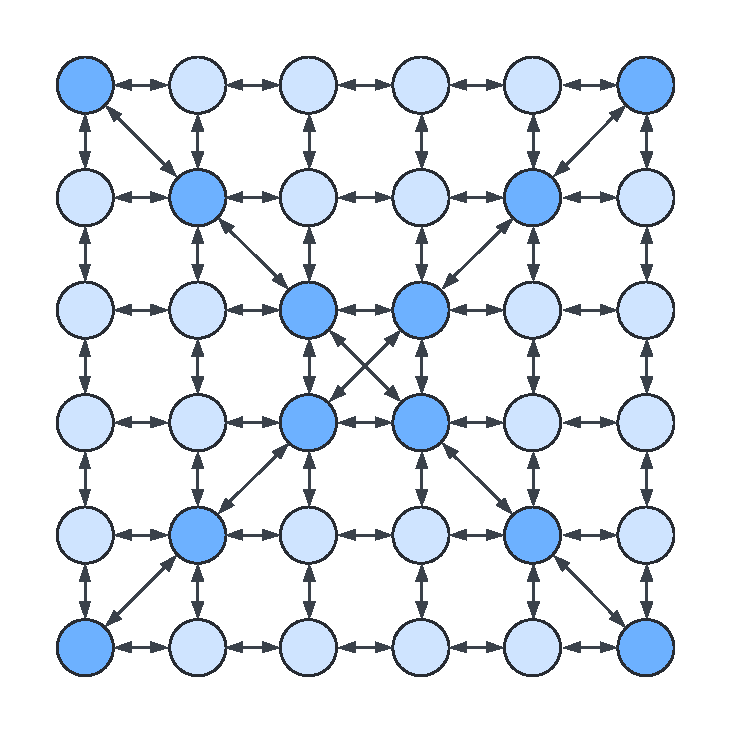
\includegraphics[width=0.45\textwidth]{assets/xdmesh_topology.pdf}
\caption{
An 6x6 XDMesh topology.
The darker blue shaded nodes feature additional diagonal links.
}
\label{fig:xdmesh_topology}
\end{figure}

Additionally, the extended diagonal mesh (XDMesh) has been proposed as an enhancement to the 2D mesh topology \cite{furhadExtendedDiagonalMesh2015}.
XDMesh improves the 2D mesh by incorporating diagonal links (see example in \cref{fig:xdmesh_topology}), which decrease the network diameter---the longest distance between two nodes situated at opposite diagonal corners of the 2D mesh.
This reduction in network diameter leads to lower communication delays and fewer  hop counts.
Experimental results show that XDMesh achieves over $40\%$ better throughput and latency compared to the 2D mesh.
Furthermore, it outperforms the 2D mesh in terms of energy efficiency, with minimal differences in silicon area.
The experimental environment makes use of the uniform traffic model, where each node in the network generates and sends data packets to all other nodes with equal probability.
In the case of the GrAICore, the nodes (i.e., the neuron cores) do not use the config NoC for intercommunication.
For this reason, the employed uniform traffic model is not a representative traffic pattern for the config NoC. 
However, the relatively small topology change introduced by XDMesh can still be worthwhile to consider for improving NoC's performance.

Routing algorithms play a vital role in determining the efficiency of data transmission in NoCs.
Research has focused on developing novel routing algorithms to optimize performance.
For example, a study introduced a low-latency routing algorithm that exploits path diversity to achieve high bandwidth and low latency in NoC routers \cite{yangExploitingPathDiversity2012}.
Furthermore, the design of energy-efficient routing algorithms has been explored to enhance the overall power efficiency of NoCs \cite{parikhPowerAwareNoCsRouting2014}.
These routing algorithms aim to balance the trade-off between performance metrics such as throughput and latency while minimizing power consumption.
The current configuration procedure for the GrAICore transmits data packets from an external source to the destination neuron cores in a sequential manner, utilizing the X-Y routing algorithm \cite{glassTurnModelAdaptive1992}.
X-Y routing, being a non-adaptive algorithm, ensures that data packets always traverses the same path from source to destination.
Consequently, the traffic pattern remains straightforward.
At a time, there is only a single flow of data from source to destination.
Because of this, no parallel communication occurs during the configuration process and therefore the congestion is minimal.
However, if we choose to explore a NoC design or configuration procedure that involves concurrent traffic through the network, potential congestion issues may arise.
In such cases, a suitable routing algorithm must be implemented to manage and mitigate congestion effectively.

%%
% The choice of routing algorithm involves trade-offs among many parameters such as latency, throughput, power consumption, fault tolerance, load balancing, scalability, implementation complexity and avoidance of deadlocks and livelocks.
% Routing algorithms are dependent on several factors that influence their design, performance and suitability for specific applications.
% What is important to note is the traffic pattern for the current config NoC.
% A traffic pattern describes the communication behaviour, such as which nodes communicate with each other and how frequently.
% Currently, when configuration happens, data is only sent sequentially from the external source to the destination neuron core.
% Furthermore, since the config NoC makes use of XY routing, the data packets all travel the same path from source to destination.
% This suggests that there are no intercommunication between neuron cores and therefore no congestion can occur due to the absence of resource (e.g., router) contention.
%%

% The current configuration procedure for the GrAICore transmits data packets from the external source to the destination neuron cores in a sequential manner, utilizing the X-Y routing algorithm.
% X-Y routing, being a non-adaptive algorithm, ensures that data packets always traverses the same path from source to destination.
% Consequently, the traffic pattern remains straightforward.
% Since no parallel communication occurs during the configuration process, congestion is minimal.

Switching techniques in NoCs play a crucial role in determining how data packets are forwarded within the network, thereby influencing latency and power consumption.
Research has proposed energy-efficient reconfigurable circuit-switched NoCs as a means to optimize power utilization while maintaining high performance \cite{wolkotteEnergyEfficientReconfigurableCircuitSwitched2005}.
Additionally, studies on switching techniques with reduced buffer requirements highlight the importance of balancing performance and power efficiency in modern NoC designs \cite{requenaEfficientSwitchingTechnique2008}.
By implementing efficient switching mechanisms, designers can achieve lower power consumption without compromising network performance.

Link width is another essential design parameter that influences the data transfer rate and overall bandwidth of the network.
Wider links can accommodate higher data rates, leading to improved throughput and reduced latency.
However, the use of wider links also consume more power, so there is a trade-off between performance and power consumption that designers need to consider when designing a NoC \cite{manhokimNetworkonchipLinkAnalysis2006}.
Widening the link widths in the GrAICore's current config NoC is a relatively straightforward enhancement, making it an appealing solution for improving both throughput and latency.
However, it is important to note that increasing the link widths also requires more silicon area due to the need for additional physical wires and increased router complexity.

% In conclusion, the current state of NoC research highlights the critical role of topology, routing algorithms, switching techniques, and link width in optimizing network performance in terms of throughput, latency, and power consumption.
% By leveraging innovative topologies, efficient routing algorithms, energy-efficient switching techniques, and appropriate link widths, designers can tailor NoC architectures to meet the increasing demands of multi-core SoCs.
% Future research in this field is likely to continue focusing on refining these aspects to achieve even higher levels of performance in on-chip communication architectures.

% In summary, Network-on-Chip (NoC) technology is integral to modern multi-core systems-on-chip (SoCs), offering significant improvements in throughput, latency, and power efficiency. The performance of NoCs is influenced by factors such as topology, routing algorithms, switching techniques, and link width. Innovations like the XDMesh topology and efficient routing algorithms demonstrate the potential for substantial gains in network performance. Switching techniques and link width adjustments further contribute to optimizing power consumption and data transfer rates. As research progresses, these advancements will continue to evolve, enabling NoC architectures to meet the growing demands of multi-core SoCs and achieve even greater levels of performance in on-chip communication.

In conclusion, NoC technology has emerged as a vital component in modern multi-core SoCs, providing high throughput, low latency, and efficient power utilization.
The performance of NoCs is shaped by several key factors, including topology, routing algorithms, switching mechanisms, and link width.
Research has highlighted the importance of selecting the right topology, such as the XDMesh, which can significantly enhance performance by reducing communication delays and hop counts.
Efficient routing algorithms and switching techniques further optimize data transmission and power efficiency.
Additionally, adjusting link widths offers a means to improve throughput and latency, though it must be balanced against increased power consumption and silicon area.
% \section{External memory}

Selecting the appropriate memory technology is critical for optimizing performance and energy efficiency.
For example, DRAM (Dynamic Random Access Memory) and NVM (Non-Volatile Memory) each present unique advantages: DRAM is known for its high speed and throughput, making it suitable for performance-intensive tasks, while NVM offers non-volatility and energy efficiency, ideal for data persistence and energy-conscious applications.
Advanced techniques such as burst transfers and parallel data interfaces can further enhance memory system performance.
Additionally, optimizing both the memory controller and Network-on-Chip (NoC) for energy efficiency is essential to achieve balanced, high-performing many-core architectures.

DRAM technology is a prevalent choice for main memory in many-core systems due to its high density and cost-effectiveness \cite{oExploringEnergyefficientDRAM2011}. Furthermore, DRAM offers fast access times and high throughput, making it suitable for applications necessitating real-time data processing. Its ability to rapidly read and refresh data contributes to its widespread adoption in performance-critical environments.
Conversely, NVM technologies provide non-volatility, high capacity, and energy efficiency, making them ideal for storing large data volumes in edge devices. NVM technologies, such as Flash memory and emerging solutions like Phase-Change Memory (PCM), present a compelling alternative to traditional volatile memory.
While DRAM excels in performance, NVM technologies are increasingly competitive and offer a compelling alternative, particularly in scenarios prioritizing energy efficiency and data persistence \cite{dulloorSystemSoftwarePersistent2014}.

PCM (Phase-Change Memory) is a notable NVM technology that leverages the unique properties of chalcogenide glass to store data \cite{meenaOverviewEmergingNonvolatile2014}.
PCM operates by changing the state of the material between amorphous and crystalline phases, which correspond to different resistance levels representing binary data.
One of the significant advantages of PCM is its superior read performance compared to traditional Flash memory.
PCM can achieve read latencies comparable to DRAM \cite{wangExploringHybridMemory2013}, making it suitable for read-intensive applications where quick data retrieval is critical.
Moreover, PCM's endurance and reliability are notable.
Unlike DRAM, which requires periodic refreshing to maintain data integrity, PCM retains data without power, significantly reducing energy consumption in standby modes.

Burst transfers play a crucial role in improving the performance of external memory systems.
By allowing for the transfer of a block of data in a single contiguous sequence, burst transfers reduce the overhead associated with individual data transfers, thereby enhancing throughput \cite{bakhodaDesigningOnchipNetworks2013}.

To further enhance performance, utilizing multiple external memory interfaces for parallel data transfers can improve overall throughput.
By enabling simultaneous data transfers through different interfaces, the system can leverage parallelism to maximize memory bandwidth utilization, particularly beneficial in many-core architectures with multiple cores accessing external memory concurrently \cite{chenIncreasingOffchipBandwidth2014}.

In the context of energy consumption, both external memory and the NoC contribute significantly to the overall power consumption of the system.
The memory controller, which manages data transfers between the processor and external memory, consumes a considerable amount of energy \cite{udipiRethinkingDRAMDesign2010}.
Additionally, the NoC, which facilitates communication between cores in a many-core chip, may also consumes a substantial portion of the system's energy budget \cite{ziaHighlyscalable3DCLOS2010}.
Optimizing the design of the memory controller and the NoC for energy efficiency is crucial for enhancing the overall energy performance of many-core systems.

When considering the integration of external memory with a NoC in a many-core chip, it is essential to address performance metrics such as throughput, latency, and energy consumption.
The choice between DRAM and NVM technologies for external memory impacts these metrics significantly, with NVM technologies offering potential advantages in terms of energy efficiency.
Burst transfers and parallel data transfer interfaces are key mechanisms for improving throughput in external memory systems, while optimizing the energy consumption of the memory controller and the NoC is vital for enhancing the overall energy efficiency of many-core systems at the edge.

% \section{GrAICore}

One of these edge AI accelerators is the GrAICore designed by GrAI Matter Labs (GML).
The GrAICore utilizes the ``NeuronFlow'' technology, a many-core architecture that is inspired by the neural structures of the brain \cite{moreiraNeuronFlowNeuromorphicProcessor2020}, \cite{moreira_neuronflow_2020}.
Its main use case is computer vision applications using models based on convolutional neural networks (CNNs).
It features a total of 144 neuron cores, arranged in a 12 by 12 grid.
A neuron core includes a local SRAM memory for storing data such as model parameters and a processing element for performing mathematical operations (see \cref{fig:neuron_core}).

\begin{figure}[htbp]
    \centering
    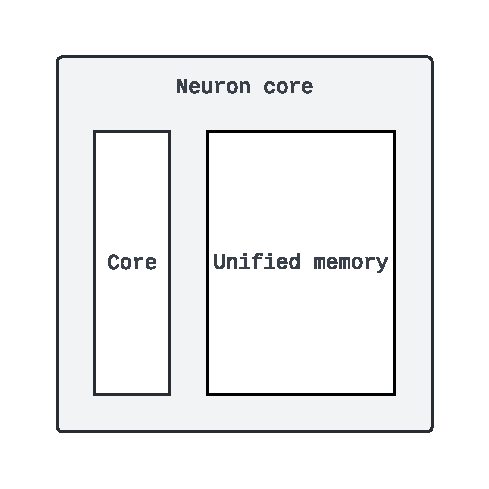
\includegraphics[width=0.25\textwidth]{assets/neuron_core.pdf}
    \caption{The neuron core includes a processing element (core) and a local memory (a.k.a. unified memory)}
    \label{fig:neuron_core}
\end{figure}

\subsubsection{Near-memory computing}
The GrAICore makes use of near-memory computing.
Near-memory computing refers to an computer architecture where computation is performed close to the memory.
This approach aims to mitigate the ``von Neumann bottleneck'', a limitation caused by the traditional computing architecture where the CPU (Central Processing Unit) and memory are separate entities, and data must be transferred back and forth between them \cite{indiveriMemoryInformationProcessing2015}.
By performing computations closer to where data is stored, data movement between the processing element and memory is minimized, reducing latency and energy consumption.
However, this introduces a constraint that requires the parameters of a model to reside in local memory before it can be used by the processing element.
Thus, an AI model must first be mapped and loaded onto the GrAICore before it can be used for inference.
Mapping means to assign the layers of a neural network to the neuron cores.
Intelligent mapping is important for balancing memory, computation and traffic between neuron cores.
The GrAICore features a total of \SI{36}{MB} of local memory, which is evenly distributed across its $144$ neuron cores.
The size of an AI model can be quantified by the number of its parameters.
For instance, if a parameter is stored as a 16-bit value on the GrAICore, it can accommodate approximately $\frac{\SI{36}{MiB}}{\SI{16}{b}}$ parameters\footnote{In practice, the available space for parameters is smaller because a portion of the memory is allocated for storing other relevant data.}, which translates to around \SI{19}{M} parameters in total.
Popular computer vision models like ResNet-50 \cite{heDeepResidualLearning2015} and YOLOv7 \cite{wangYOLOv7TrainableBagoffreebies2022}, with over \SI{25}{M} and \SI{37}{M} parameters respectively, are already too large by themselves to fit on the GrAICore.
Using optimization techniques, these models can be compressed into a smaller size.
For example, YOLOv7-tiny \cite{wangYOLOv7TrainableBagoffreebies2022} is a size optimized model of the YOLOv7 for edge devices at the cost of accuracy.
Its size is decreased to around \SI{6}{M} parameters, making it suitable for the GrAICore.
In summary, the number of parameters that can be stored on the GrAICore is limited by the size of its memory.
% Due to this, the GrAICore is only able to support limited sized AI models.

\begin{figure}[htbp]
    \centering
    \subfloat[The event NoC features a 2D torus topology]{
        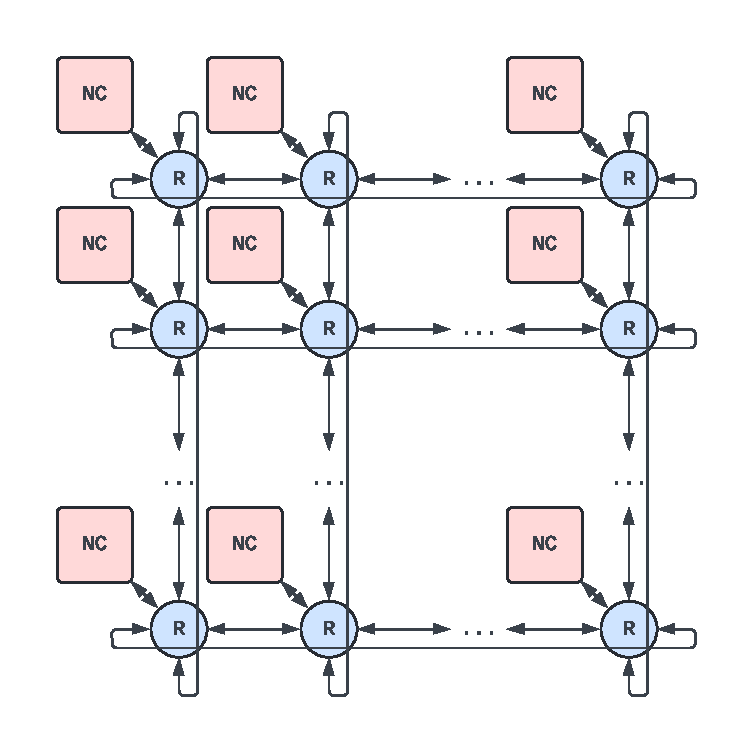
\includegraphics[width=0.45\textwidth]{assets/event_noc.pdf}
        \label{fig:event_noc}
    }
    \hfill
    \subfloat[The config NoC features a 2D mesh topology]{
        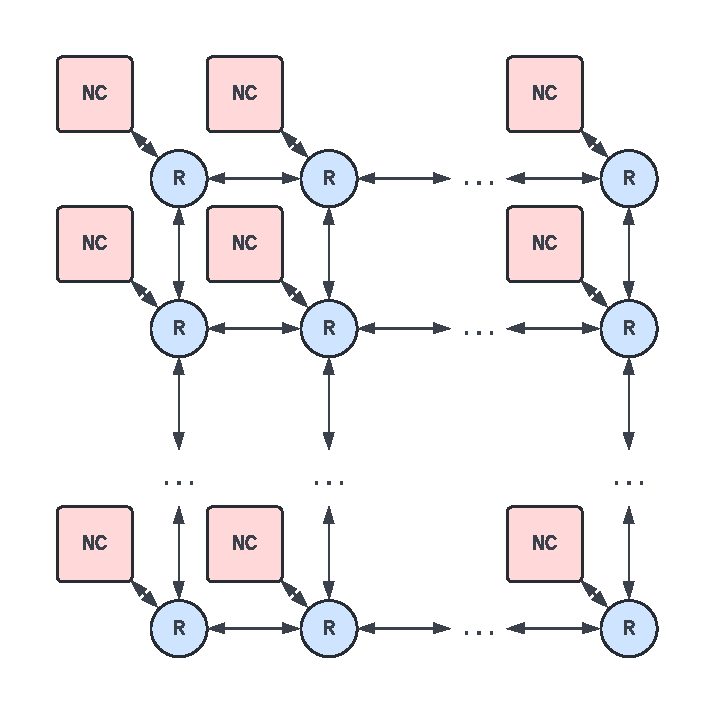
\includegraphics[width=0.45\textwidth]{assets/config_noc.pdf}
        \label{fig:config_noc}
    }
    \caption{GrAICore's network-on-chips. A neuron core (NC) communicates via its associated router (R) with other neuron cores and external parties such as the host device (not illustrated).}
    \label{fig:noc}
\end{figure}

\subsubsection{NoCs}
The neuron cores are connected to each other with two distinct network-on-chips (NoCs), each serving its own purpose (see \cref{fig:noc}).
% Firstly, the event NoC is responsible for transferring small packets of data called Events to its destination.
Firstly, the event NoC is used for exchanging activated neuron states in the form of small messages called Events.
Events are only generated when an AI model is being executed.
The event NoC uses the 2D torus topology.
Secondly, the config NoC is responsible for configuring the GrAICore, monitoring and debugging.
The config NoC uses a different topology, namely a 2D mesh topology.
Configuring the GrAICore means that the local memories of the neuron cores are written with the parameters of an AI model.
A host device (e.g., a microcontroller) initiates the configuration of the GrAICore.
The host device is connected to the config NoC via a single link, which is used to transfer data to and from any neuron core.
Since all data transfers must go through this link to reach its destination neuron core, it causes a significant bottleneck in data transfer speed to the GrAICore.
That is, the amount of data that can be transferred to the neuron cores within a certain time is poor as it was not designed with speed in mind.
Therefore, currently, the configuration of the memories of the neuron cores is only performed once at the start.
% This limitation restricts the GrAICore to be (partially) reconfigured at run-time.


% \section{Swapping}

A technique that is similar to our plan of action is called swapping.
Swapping involves dynamically loading and unloading part of the model or data into and out of the device’s memory during inference or execution time \cite{wangSwapNetEfficientSwapping2024, huangSwapAdvisorPushingDeep2020}.
\cite{wang_swapnet_2024, huang_swapadvisor_2020}
When a large model cannot fit in the device’s memory. Parts of the model (e.g., layers) are stored in slower, but larger storage.
These parts are then loaded into the device’s memory on-demand during execution.
The device is responsible for scheduling the execution of the model parts so that the necessary chunks are loaded into the device’s memory in time for computation.
This will require careful timing to ensure that data is ready when needed to avoid stalling the processor.
Swapping introduces latency, as loading data from the slower storage takes time.
It is therefore crucial that this overhead is minimized to ensure that performance is acceptable.

Research has been done on using the swapping technique for supporting large neural networks on tiny microcontrollers in \cite{miaoEnablingLargeNeural2021}.
This is achieved by dynamically swapping neural network parts between a microcontroller's tiny SRAM and its large, low-cost external flash.
Although they managed to address the challenge of running large models on a resource-constrained edge device without accuracy loss, a microcontroller's hardware architecture is significantly different compared to that of the GrAICore's.
With low-cost microcontrollers as their target, the external flash bandwidth is usually poor ($<\SI{100}{MB/s}$).
As a consequence, the throughput of processed frames per second is also poor.
But despite that, the proposed scheduling technique shows promising results for executing large models on microcontrollers and can potentially be extended to be used on the GrAICore.




% \section{Requirements analysis}
There is a need to integrate external memory access into the GrAICore's architecture.
The addition of the external memory extends the total memory of system, allowing the system to store larger and multiple AI models.
The access to the external memory must be efficient in terms of throughput and power.
The external memory, along with the GrAICore’s architecture, must provide a sufficiently high data transfer rate to load the GrAICore with a new (partial) AI model seamlessly.

We consider two separate cases:
\begin{itemize}
    \item \textbf{Multiple models}: here we assume that the AI models are all exactly the size of the memory capacity of the GrAICore.
    This implies that the complete memory of the GrAICore must be written to load a new AI model.
    \item \textbf{Large model}: a large AI model is too large to be fitted onto the GrAICore's memory at once.
    Therefore, a large AI model must be run in parts by partitioning the model into smaller pieces.
\end{itemize}

\subsubsection{Multiple models}
The GrAICore is unable to make use of multiple models as they do not fit in the local memories simultaneously.
Additionally, the GrAICore lacks the ability to reconfigure itself during run-time.
The time it takes to process a frame is dependent on the complexity of the model on the GrAICore.
Based on realistic use-cases with models executed on the GrAICore, it has been established by GML that the processing time of a frame takes up to \SI{5}{ms} for a representative application.
For a video with a frame rate of $\SI{60}{FPS}$, there is a period of $\SI{16.7}{ms}$ between two frames (called the frame time).
Within this period, the succeeding frame will be processed.
Thus, for a video with a frame rate of $\SI{60}{FPS}$, we have a maximum reconfiguration time budget of $\SI{11.7}{ms}$ to seamlessly reconfigure the GrAICore.
For the target frame rate of \SI{60}{FPS}, where each frame must be processed within approximately \SI{11.7}{ms}, there is no need for pipelining of frames since the frame processing time consistently fits within this time budget.
In this specific context, increasing the throughput of processed frames through pipelining does not provide additional benefits, as the system is already capable of handling each frame within the required interval.

Clearly, an increase in frame rate ($f$) decreases the available time budget ($B$) for reconfiguration (see \cref{fig:fps_vs_budget}):
\begin{equation}
    B = f^{-1} - \SI{5}{ms}
\end{equation}

\begin{figure}[htbp]
    \centering
    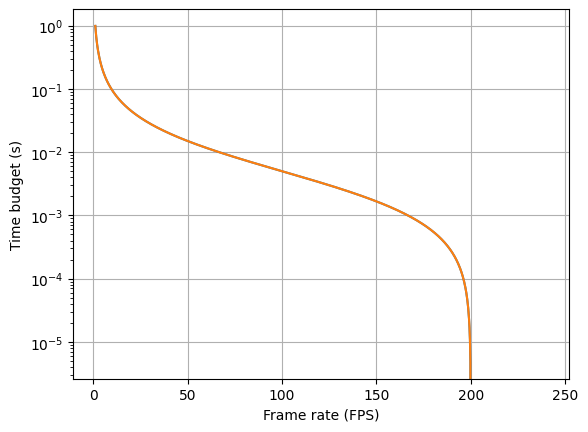
\includegraphics[width=0.5\linewidth]{assets/fps_vs_budget.png}
    \caption{An increase in frame rate lowers the maximum reconfiguration time budget}
    \label{fig:fps_vs_budget}
\end{figure}

\begin{table}[htbp]
\centering
\begin{tabular}{@{}lll@{}}
\toprule
Frame rate (FPS) & Frame time (ms) & Reconf. budget (ms) \\ \midrule
15               & 66.7            & 61.7                \\
24               & 41.7            & 36.7                \\
30               & 33.3            & 28.3                \\
60               & 16.7            & 11.7                \\
120              & 8.3             & 3.3                 \\
200              & 5               & 0                   \\
240              & 4.2             & -0.8                \\ \bottomrule
\end{tabular}
\caption{Reconfiguration time budget for different common video frame rates. The frame times and reconfiguration budgets are rounded.}
\label{tab:common_fps}
\end{table}

\Cref{tab:common_fps} shows a list of common video frame rates with their associated reconfiguration time budget.
A frame rate with zero or negative time budget means that the GrAICore cannot be reconfigured seamlessly for a video with that frame rate.
Exceeding this time budget results into a delayed output which is undesirable since it negatively affects the user experience.
At a frame rate of $\SI{200}{FPS}$, the time budget is exactly zero, indicating that this represents the tight upper bound.
\Cref{fig:reconfig_time_line_ex} shows two time lines exemplifying a seamless and non-seamless reconfiguration procedure.

In terms of bandwidth, to reconfigure the GrAICore fully (i.e., write all $\SI{36}{MB}$ of local memory), we require a minimum of $\SI{3086}{MB/s}$\footnote{$\frac{36}{\frac{1}{60} - 5 \times 10^{-3}} \approx 3086$} for $\SI{60}{FPS}$.
Note that this bandwidth number does not include any overhead induced by communication protocols. Therefore, in practice, the required minimum bandwidth is higher. 

With a technique such as layer-by-layer replacement, pipelining of configuration and processing can be achieved \cite{jiDemandLayeringRealTime2022}.
However, there are a multitude of challenges associated with this technique. 
Firstly, the sizes of an old (already processed) layer and a new (to be replaced with) layer may differ.
Replacing a layer is straightforward when the new layer is equal or smaller in size.
However, if the new layer is larger in size, it cannot fit as a whole.
It will need to replace multiple old layers to able to fit.
Secondly, the system will need a way to notify the relevant parties that a specific layer has completed processing.
This is required for indicating that a layer (or multiple layers) can be replaced by a new one. %synchronization
Finally, the time it takes to process a layer has not been explored before.
This is crucial to provide us a number that can be used to determine the reconfiguration time budget.
Due to these additional complexities, we have opted not to consider this technique.
Furthermore, we only consider the scenario where each frame is processed by a single model and reconfiguration may only happen whenever a frame has finished processing.

\begin{figure}[htbp]
    \centering
    \subfloat[]{
        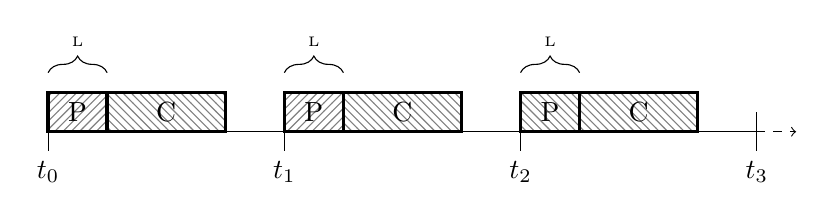
\begin{tikzpicture}[scale=0.5]
    \draw[] (6,0) -- (24,0);
    \draw[dashed, ->] (24,0) -- (25,0);
    \draw (6,0.5) -- (6,-0.5) node[below] {$t_{0}$};
    \draw (12,0.5) -- (12,-0.5) node[below] {$t_{1}$};
    \draw (18,0.5) -- (18,-0.5) node[below] {$t_{2}$};
    \draw (24,0.5) -- (24,-0.5) node[below] {$t_{3}$};

    \draw [pattern=north east lines, pattern color=gray, line width = 1pt, very thick] ($(6,0)$) rectangle ++($(1.5,1)$) node[midway] {P};
    \draw [pattern=north west lines, pattern color=gray, line width = 1pt, very thick] ($(7.5,0)$) rectangle ++($(3,1)$) node[midway] {C};
    \draw [decorate,decoration={brace,amplitude=6pt}]($(6,1.5)$) -- ++($(1.5,0)$) node [black,midway,above=6pt] {\tiny L};
    
    \draw [pattern=north east lines, pattern color=gray, line width = 1pt, very thick] ($(12,0)$) rectangle ++($(1.5,1)$) node[midway] {P};
    \draw [pattern=north west lines, pattern color=gray, line width = 1pt, very thick] ($(13.5,0)$) rectangle ++($(3,1)$) node[midway] {C};
    \draw [decorate,decoration={brace,amplitude=6pt}]($(12,1.5)$) -- ++($(1.5,0)$) node [black,midway,above=6pt] {\tiny L};
    
    \draw [pattern=north west lines, pattern color=gray, line width = 1pt, very thick] ($(18,0)$) rectangle ++($(1.5,1)$) node[midway] {P};
    \draw [pattern=north west lines, pattern color=gray, line width = 1pt, very thick] ($(19.5,0)$) rectangle ++($(3,1)$) node[midway] {C};
    \draw [decorate,decoration={brace,amplitude=6pt}]($(18,1.5)$) -- ++($(1.5,0)$) node [black,midway,above=6pt] {\tiny L};
\end{tikzpicture}

        \label{fig:correct_reconfig}
    } \\
    \subfloat[]{
        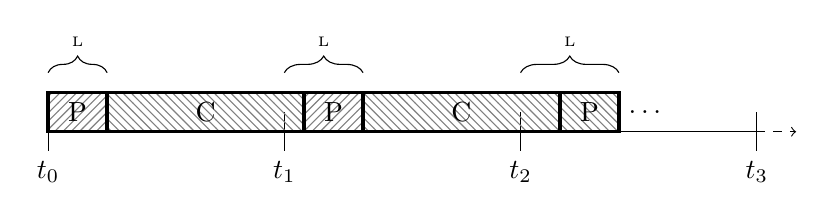
\begin{tikzpicture}[scale=0.5]
    \draw[] (6,0) -- (24,0);
    \draw[dashed, ->] (24,0) -- (25,0);
    \draw (6,0.5) -- (6,-0.5) node[below] {$t_{0}$};
    \draw (12,0.5) -- (12,-0.5) node[below] {$t_{1}$};
    \draw (18,0.5) -- (18,-0.5) node[below] {$t_{2}$};
    \draw (24,0.5) -- (24,-0.5) node[below] {$t_{3}$};

    \draw [pattern=north east lines, pattern color=gray, line width = 1pt, very thick] ($(6,0)$) rectangle ++($(1.5,1)$) node[midway] {P};
    \draw [pattern=north west lines, pattern color=gray, line width = 1pt, very thick] ($(7.5,0)$) rectangle ++($(5,1)$) node[midway] {C};
    \draw [decorate,decoration={brace,amplitude=6pt}]($(6,1.5)$) -- ++($(1.5,0)$) node [black,midway,above=6pt] {\tiny L};
    
    \draw [pattern=north east lines, pattern color=gray, line width = 1pt, very thick] ($(12.5,0)$) rectangle ++($(1.5,1)$) node[midway] {P};
    \draw [pattern=north west lines, pattern color=gray, line width = 1pt, very thick] ($(14,0)$) rectangle ++($(5,1)$) node[midway] {C};
    \draw [decorate,decoration={brace,amplitude=6pt}]($(12,1.5)$) -- ++($(2,0)$) node [black,midway,above=6pt] {\tiny L};
    
    \draw [pattern=north west lines, pattern color=gray, line width = 1pt, very thick] ($(19,0)$) rectangle ++($(1.5,1)$) node[midway] {P};
    % \draw [pattern=north west lines, pattern color=gray, line width = 1pt, very thick] ($(20.5,0)$) rectangle ++($(5,1)$) node[midway] {C};
    \draw [decorate,decoration={brace,amplitude=6pt}]($(18,1.5)$) -- ++($(2.5,0)$) node [black,midway,above=6pt] {\tiny L};
    \node[right] at (20.5,0.5) {\ldots};



\end{tikzpicture}
        \label{fig:incorrect_reconfig}
    }
    \caption{
    Example time lines of reconfiguration procedures.
    $t_n$ indicates the time instance where the $n$th frame has been received by the GrAICore, ready to be processed.
    At $t_0$, the GrAICore is already configured with an initial model.
    In \protect\subref{fig:correct_reconfig}, the GrAICore uses a different model for each consecutive frame.
    After receiving and processing (P) the very first frame at $t_0$, it starts reconfiguration (C) to a new model.
    Since the sum of the reconfiguration and processing time does not exceed the frame time ($t_{n+1} - t_{n})$, the frame processing latency (L) is equal for every incoming frame.
    The invariant latency is desired and indicates a seamless reconfiguration.
    \protect\subref{fig:incorrect_reconfig} has an increased reconfiguration time.
    Now, the sum of the reconfiguration and processing time does exceed the frame time.
    As a consequence, the frame processing latency increases for each incoming frame.
    In the long run, this latency will grow to infinity.
    Since the latency varies, this is an example of a non-seamless reconfiguration.
    }
    \label{fig:reconfig_time_line_ex}
\end{figure}

\subsubsection{Large model}

Due to the GrAICore having limited memory capacity, a single large model cannot be loaded onto it at once.
Several works have proposed strategies for deploying CNNs on resource-constrained devices.
Among these strategies, "partitioning" refers to splitting an entire model at specific locations to create one or more partitions, thereby reducing instantaneous memory requirements \cite{kaboubiHybridPartitioningEmbedded2023}.
To fully process a frame, one or more (partial) reconfigurations will need to be performed.
Each of the reconfigurations will load in the subsequent neural network part needed for further processing.

For this case, a specific timing or bandwidth cannot be as easily determined.
This is due to the nature of a large model. A large model can be of any arbitrary size.
With a larger model having to be partitioned into more parts.
Consequently, an increase in parts sees an increase in the amount of reconfigurations necessary to execute the large model completely.
Due to this, determining the total reconfiguration time budget is more involved.
A single frame is ``processed'' multiple times, once by each part of the neural network.
The total reconfiguration time budget is dependent on the number of (partial) reconfigurations necessary to fully process a single frame.

\begin{table}[hbtp]
\centering
\begin{tabular}{@{}lllllll@{}}
\toprule
    &            & \multicolumn{5}{l}{Time budget per reconfiguration amount (ms)} \\
FPS & Frame time (ms) & 1x         & 2x          & 3x         & 4x         & 5x         \\ \midrule
5   & 200  & 195  & 190  & 185  & 180   & 175   \\
15  & 66.7 & 61.7 & 56.7 & 51.7 & 46.7  & 41.7  \\
24  & 41.7 & 36.7 & 31.7 & 26.7 & 21.7  & 16.7  \\
30  & 33.3 & 28.3 & 23.3 & 18.3 & 13.3  & 8.3   \\
60  & 16.7 & 11.7 & 6.7  & 1.7  & -3.3  & -8.3  \\
120 & 8.3  & 3.3  & -1.7 & -6.7 & -11.7 & -16.7 \\ \bottomrule
\end{tabular}
\caption{Maximum reconfiguration time budget for common frame rates and different reconfiguration amounts. The frame times and time budgets are rounded.}
\label{tab:common_fps_reconfig_amount}
\end{table}

As an example, assume that a large model is partitioned into an arbitrary amount of parts.
Each part is exactly the size of the GrAICore's total capacity and the processing time for each part takes $\SI{5}{ms}$.
\Cref{tab:common_fps_reconfig_amount} shows that for a video of $\SI{60}{FPS}$ and a large model requiring two reconfigurations, we have a maximum reconfiguration time budget of $\SI{6.7}{ms}$.
Notice that a large model that requires $4$ reconfigurations at \SI{60}{FPS} has a negative time budget.
This means that it is not possible to process a frame for a video of \SI{60}{FPS} within two consecutive incoming frames for that particular model.
Processing frames at \SI{60}{FPS} with a large model is often not feasible, as many models require more than a few reconfigurations.
A lower frame rate gives us a larger reconfiguration budget, which is more suitable for larger models.
Notably, reducing the frame rate to single digits significantly increases the available reconfiguration budget.
\Cref{fig:larger_reconfig_ex} illustrates two time lines showing a good and a bad scenario.

\begin{figure}[htbp]
    \centering
    \subfloat[]{
        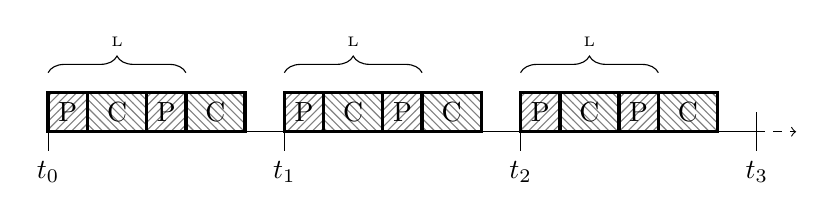
\begin{tikzpicture}[scale=0.5]

    \draw[] (6,0) -- (24,0);
    % \draw[dashed, <-] (5,0) -- (6,0);
    \draw[dashed, ->] (24,0) -- (25,0);
    \draw (6,0.5) -- (6,-0.5) node[below] {$t_{0}$};
    \draw (12,0.5) -- (12,-0.5) node[below] {$t_{1}$};
    \draw (18,0.5) -- (18,-0.5) node[below] {$t_{2}$};
    \draw (24,0.5) -- (24,-0.5) node[below] {$t_{3}$};
    
    \draw [pattern=north east lines, pattern color=gray, line width = 1pt, very thick] ($(6,0)$) rectangle ++($(1,1)$) node[midway] {P};
    \draw [pattern=north west lines, pattern color=gray, line width = 1pt, very thick] ($(7,0)$) rectangle ++($(1.5,1)$) node[midway] {C};
    \draw [pattern=north east lines, pattern color=gray, line width = 1pt, very thick] ($(8.5,0)$) rectangle ++($(1,1)$) node[midway] {P};
    \draw [pattern=north west lines, pattern color=gray, line width = 1pt, very thick] ($(9.5,0)$) rectangle ++($(1.5,1)$) node[midway] {C};
    \draw [decorate,decoration={brace,amplitude=6pt}]($(6,1.5)$) -- ++($(3.5,0)$) node [black,midway,above=6pt] {\tiny L};
    
    \draw [pattern=north east lines, pattern color=gray, line width = 1pt, very thick] ($(12,0)$) rectangle ++($(1,1)$) node[midway] {P};
    \draw [pattern=north west lines, pattern color=gray, line width = 1pt, very thick] ($(13,0)$) rectangle ++($(1.5,1)$) node[midway] {C};
    \draw [pattern=north east lines, pattern color=gray, line width = 1pt, very thick] ($(14.5,0)$) rectangle ++($(1,1)$) node[midway] {P};
    \draw [pattern=north west lines, pattern color=gray, line width = 1pt, very thick] ($(15.5,0)$) rectangle ++($(1.5,1)$) node[midway] {C};
    \draw [decorate,decoration={brace,amplitude=6pt}]($(12,1.5)$) -- ++($(3.5,0)$) node [black,midway,above=6pt] {\tiny L};
    
    \draw [pattern=north east lines, pattern color=gray, line width = 1pt, very thick] ($(18,0)$) rectangle ++($(1,1)$) node[midway] {P};
    \draw [pattern=north west lines, pattern color=gray, line width = 1pt, very thick] ($(19,0)$) rectangle ++($(1.5,1)$) node[midway] {C};
    \draw [pattern=north east lines, pattern color=gray, line width = 1pt, very thick] ($(20.5,0)$) rectangle ++($(1,1)$) node[midway] {P};
    \draw [pattern=north west lines, pattern color=gray, line width = 1pt, very thick] ($(21.5,0)$) rectangle ++($(1.5,1)$) node[midway] {C};
    \draw [decorate,decoration={brace,amplitude=6pt}]($(18,1.5)$) -- ++($(3.5,0)$) node [black,midway,above=6pt] {\tiny L};
\end{tikzpicture}

        \label{fig:large_reconfig_ex1}
    } \\
    \subfloat[]{
        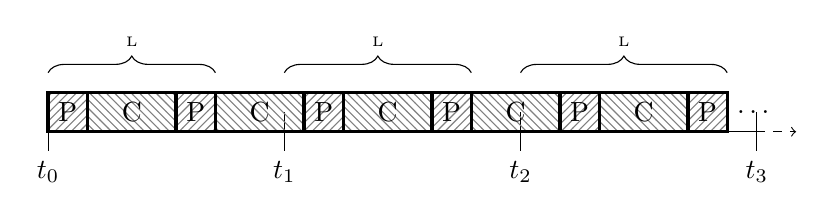
\begin{tikzpicture}[scale=0.5]

    \draw[] (6,0) -- (24,0);
    \draw[dashed, ->] (24,0) -- (25,0);
    \draw (6,0.5) -- (6,-0.5) node[below] {$t_{0}$};
    \draw (12,0.5) -- (12,-0.5) node[below] {$t_{1}$};
    \draw (18,0.5) -- (18,-0.5) node[below] {$t_{2}$};
    \draw (24,0.5) -- (24,-0.5) node[below] {$t_{3}$};
    
    \draw [pattern=north east lines, pattern color=gray, line width = 1pt, very thick] ($(6,0)$) rectangle ++($(1,1)$) node[midway] {P};
    \draw [pattern=north west lines, pattern color=gray, line width = 1pt, very thick] ($(7,0)$) rectangle ++($(2.25,1)$) node[midway] {C};
    \draw [pattern=north east lines, pattern color=gray, line width = 1pt, very thick] ($(9.25,0)$) rectangle ++($(1,1)$) node[midway] {P};
    \draw [pattern=north west lines, pattern color=gray, line width = 1pt, very thick] ($(10.25,0)$) rectangle ++($(2.25,1)$) node[midway] {C};
    \draw [decorate,decoration={brace,amplitude=6pt}]($(6,1.5)$) -- ++($(4.25,0)$) node [black,midway,above=6pt] {\tiny L};
    
    \draw [pattern=north east lines, pattern color=gray, line width = 1pt, very thick] ($(12.5,0)$) rectangle ++($(1,1)$) node[midway] {P};
    \draw [pattern=north west lines, pattern color=gray, line width = 1pt, very thick] ($(13.5,0)$) rectangle ++($(2.25,1)$) node[midway] {C};
    \draw [pattern=north east lines, pattern color=gray, line width = 1pt, very thick] ($(15.75,0)$) rectangle ++($(1,1)$) node[midway] {P};
    \draw [pattern=north west lines, pattern color=gray, line width = 1pt, very thick] ($(16.75,0)$) rectangle ++($(2.25,1)$) node[midway] {C};
    \draw [decorate,decoration={brace,amplitude=6pt}]($(12,1.5)$) -- ++($(4.75,0)$) node [black,midway,above=6pt] {\tiny L};
    
    \draw [pattern=north east lines, pattern color=gray, line width = 1pt, very thick] ($(19,0)$) rectangle ++($(1,1)$) node[midway] {P};
    \draw [pattern=north west lines, pattern color=gray, line width = 1pt, very thick] ($(20,0)$) rectangle ++($(2.25,1)$) node[midway] {C};
    \draw [pattern=north east lines, pattern color=gray, line width = 1pt, very thick] ($(22.25,0)$) rectangle ++($(1,1)$) node[midway] {P};
    % \draw [pattern=north west lines, pattern color=gray, line width = 1pt, very thick] ($(23.25,0)$) rectangle ++($(2.25,1)$) node[midway] {C};
    \node[right] at (23.25,0.5) {\ldots};
    \draw [decorate,decoration={brace,amplitude=6pt}]($(18,1.5)$) -- ++($(5.25,0)$) node [black,midway,above=6pt] {\tiny L};

\end{tikzpicture}
        \label{fig:large_reconfig_ex2}
    }
    \caption{
        Example time lines of processing a large model requiring two reconfigurations.
        At $t_0$, the GrAICore is already configured with the first part of the model.
        In \protect\subref{fig:large_reconfig_ex1}, the two reconfiguration periods (C) and two processing periods (P) fit within the reception of two consecutive frames ($t_n$ and $t_{n+1}$).
        The frame processing latency (L) is equal for every incoming frame.
        In \protect\subref{fig:large_reconfig_ex2}, the reconfiguration time is increased. 
        This results into an ever-increasing frame processing latency.
    }
    \label{fig:larger_reconfig_ex}
\end{figure}

We will examine realistic AI models, specifically the ResNet-101 model \cite{heDeepResidualLearning2015}, which is a potential use case for the GrAICore and exceeds its local memory, to understand the required timings and bandwidth.
This analysis will provide insights into the bandwidth requirements and power usage of a large AI model.
However, given the complexity of this analysis, it will be deferred to the project phase.

\subsubsection{Power consumption}
Since the GrAICore is primarily used as an AI accelerator for edge devices, maintaining low power consumption is crucial.
The addition of external memory with the capability to reconfigure the GrAICore will inevitably increase the overall power consumption of the system.
However, specific optimizations can be implemented to minimize this increase.
The solution should encompass the memory, interface, and controller, with a focus on achieving minimal power usage.

We are considering options such as DRAM or NVM, and the final selection will balance power efficiency, performance, and system compatibility.
It has been measured that the GrAICore consumes between \SI{200}{mW} and \SI{500}{mW} when processing frames at \SI{60}{FPS}.
We aim to not exceed \SI{20}{mW} when performing 60 reconfigurations per second.


% \section{Method}
% \section{Results and analysis}
% \section{Discussion}
% \section{Conclusions and future work}
% \subsection{Conclusions}
% \subsection{Future work}

% % \section{Evaluation of the config Noc}
% \section{Introduction}
The config NoC is mainly used for configuration writes to the neuron core memories.
Another use is status monitoring reads while the GrAICore is in operation.
The config NoC is a separate NoC next to the event NoC, which is used for the execution of a model.
It connects all 144 neuron cores via a 2D mesh topology (see \cref{fig:noc}).
The network receives and forwards data using routers at each neuron core.
The config NoC has a single 16-bit wide interface for incoming data from an AXI slave.
Similarly, the links between every two adjacent routers are 16-bit wide. 
The clock frequency of the system is \SI{800}{MHz}.


\section{Architecture}
\lipsum[1]
% purpose
% topology
% 
The config NoC makes u
The config NoC incorporates a 2D 
Unlike the event NoC, the config NoC incorporates a 2D mesh topology.
The wraparound links of the event NoC provide noticeable benefits in communication performance.
In the event NoC, intercommunication happens between the neuron cores.
The presence of the wraparound links helps to drastically reduce the average amount of hops a packet has to take.
T
The wraparound links do not provide any noticeable benefits to the config NoC since these interactions do not occur with the config NoC.


\section{Network packet format}
The network makes use of network packets for data communication.
The phit size of the config NoC is 16 bits wide.
This implies that a total of 16 bits of data can be transferred over a link in a single cycle.
Each packet contains a header, made up of two separate phits.
The header contains the fields as shown in \cref{tab:header_fields}.

\begin{table}[hbtp]
\centering
\begin{tabular}{@{}ll@{}}
\toprule
\textbf{Header field} & \textbf{\# of bits} \\ \midrule
Packet type           & 2                   \\
Destination cluster X & 4                   \\
Destination cluster Y & 4                   \\
Address               & 20                  \\ \bottomrule
\end{tabular}
\caption{Header fields of a config NoC packet}
\label{tab:header_fields}
\end{table}

The \textit{packet type} field defines whether the packet is a \textit{read request}, \textit{read response} or \textit{write request} packet.
A \textit{read request} packet is initiated by the host.
It is used to retrieve data from a neuron core.
A \textit{read response} packet is produced as an answer to a \textit{read request}.
This packet contains the requested data that is sent back to the host.
Finally, the \textit{write request} is used to write data to a neuron core.

Both the \textit{read response} and \textit{write request} packets has two phits following the header (see \cref{fig:read_response_packet,fig:write_request_packet}).
These two phits contain the payload data that is requested.
Thus in total, packets of these two types are 64 bits in size.
The \textit{read request} packet only consists of the header (see \cref{fig:read_request_packet}).

The destination cluster coordinates are both 4 bits in size due to the need to address 12 different X and 12 different Y coordinates.

The \textit{address field} of 20 bits, allows the system to address $2^{20}$ different addresses.
This address space is used to address the SRAM and the register bank of a neuron core.
% This address space is used to address the SRAM and the register bank of a neuron core, with room to spare \cite{TODO}.

With this packet format, we observe that there is a significant overhead when writing or reading data.
For every 32 bits of data we read or write, an overhead of 32 bits is also included.
In other words, there is an overhead of $100\%$ for every read or write request of 32 bits.
At most, on average, the network transmits one byte of payload data per cycle.

% There is potential to increase this to 64 bits (or 8 bytes) per cycle which is the amount of data an SRAM in a single core can write in a single cycle.

\hspace*{0.5em}
\begin{figure}[htbp]
    \centering
    \begin{subfigure}[b]{\linewidth}
        \centering
        \begin{adjustbox}{width=0.8\linewidth}
            \begin{bytefield}[
    boxformatting={\centering\ttfamily},
    bitformatting={\ttfamily\small},
    endianness=big,
    bitwidth=2em
]{16}
\bitheader{0, 2, 6, 10, 12, 15} \\

\begin{rightwordgroup}{Header}
    \bitbox{4}[bgcolor=lightcyan]{Address[3:0]} &
    \bitbox{2}[bgcolor=lightgray]{Unused} &
    \bitbox{4}[bgcolor=lightred]{Dest. Y} &
    \bitbox{4}[bgcolor=lightorange]{Dest. X} &
    \bitbox{2}[bgcolor=lightgreen]{\scriptsize Packet type} \\
    \bitbox{16}[bgcolor=lightcyan]{Address[19:4]} &
\end{rightwordgroup}

\end{bytefield}
        \end{adjustbox}
        \caption{Read request}
        \label{fig:read_request_packet}
    \end{subfigure}
    \\ \vspace{1.5em}
    \begin{subfigure}[b]{\linewidth}
        \centering
        \begin{adjustbox}{width=0.8\linewidth}
            \begin{bytefield}[
    boxformatting={\centering\ttfamily},
    bitformatting={\ttfamily\small},
    endianness=big,
    bitwidth=2em
]{16}
\bitheader{0, 2, 6, 10, 12, 15} \\

\begin{rightwordgroup}{Header}
    \bitbox{4}[bgcolor=lightcyan]{Address[3:0]} &
    \bitbox{2}[bgcolor=lightgray]{Unused} &
    \bitbox{4}[bgcolor=lightred]{Dest. Y} &
    \bitbox{4}[bgcolor=lightorange]{Dest. X} &
    \bitbox{2}[bgcolor=lightgreen]{\scriptsize Packet type} \\

    \bitbox{16}[bgcolor=lightcyan]{Address[19:4]}
\end{rightwordgroup} \\

\begin{rightwordgroup}{Payload}
    \bitbox{16}[bgcolor=lightpurple]{Read data[15:0]} \\
    \bitbox{16}[bgcolor=lightpurple]{Read data[31:16]}
\end{rightwordgroup}

\end{bytefield}
        \end{adjustbox}
        \caption{Read response}
        \label{fig:read_response_packet}
    \end{subfigure}
    \\ \vspace{1.5em}
    \begin{subfigure}[b]{\linewidth}
        \centering
        \begin{adjustbox}{width=0.8\linewidth}
            \begin{bytefield}[
    boxformatting={\centering\ttfamily},
    bitformatting={\ttfamily\small},
    endianness=big,
    bitwidth=2em
]{16}
\bitheader{0, 2, 6, 10, 12, 15} \\

\begin{rightwordgroup}{Header}
    \bitbox{4}[bgcolor=lightcyan]{Address[3:0]} &
    \bitbox{2}[bgcolor=lightgray]{Unused} &
    \bitbox{4}[bgcolor=lightred]{Dest. Y} &
    \bitbox{4}[bgcolor=lightorange]{Dest. X} &
    \bitbox{2}[bgcolor=lightgreen]{\scriptsize Packet type} \\

    \bitbox{16}[bgcolor=lightcyan]{Address[19:4]}
\end{rightwordgroup} \\

\begin{rightwordgroup}{Payload}
    \bitbox{16}[bgcolor=lightpurple]{Write data[15:0]} \\
    \bitbox{16}[bgcolor=lightpurple]{Write data[31:16]}
\end{rightwordgroup}

\end{bytefield}
        \end{adjustbox}
        \caption{Write request}
        \label{fig:write_request_packet}
    \end{subfigure}
    \caption{
        Config NoC packet structures
    }
    \label{fig:config_noc_packets}
\end{figure}

\section{Bandwidth}
Configuration is done by transferring write request packets from the host to one or more neuron cores.
A write request packet consists of 64 bits in total.
Recall that the SRAM capacity of a single neuron core is \SI{256}{KiB}.
If we want to completely fill up one of these memories, a total of $\frac{\SI{256}{KiB}}{\SI{32}{b}} = 65536$ write request packets needs to be sent.
This means that, in total, \SI{256}{KiB} of payload data and \SI{256}{KiB} of header data is sent through the NoC.

To estimate the time to write a certain amount of data to the memories of the GrAICore, we can make use of \cref{eq:latency}.
The effective bandwidth can be calculated with \cref{eq:bandwidth}.

\begin{equation}
    T = 
    \frac{d_{\text{payload}} + d_{\text{overhead}}}
    {f_{\text{clock}} \times w_{\text{phit}}}
\label{eq:latency}
\end{equation}

\begin{equation}
    \text{BW}_{\text{eff}} =
    \frac{d_\text{payload}}{T}
\label{eq:bandwidth}
\end{equation}

\begin{eqexpl}[15mm]
    \item{$T$} time to write data
    \item{$\text{BW}_{\text{eff}}$} effective bandwidth
    \item{$d_{\text{payload}}$} amount of payload data
    \item{$d_{\text{overhead}}$} amount of overhead data
    \item{$f_{\text{clock}}$} system's clock frequency
    \item{$w_{\text{phit}}$} width of a phit
\end{eqexpl}

For example, to completely fill up the GrAICore's memory (\SI{36}{MiB}), it will take around \SI{47}{ms}\footnote{$\frac{\SI{36}{MiB} + \SI{36}{MiB}}{\SI{800}{MHz} \times \SI{16}{b}}$}.
% This translates to an effective bandwidth of $\frac{\SI{36}{MiB}}{\SI{47}{ms}} \approx \SI{763}{MiB/s}$.
This translates to an effective bandwidth of \SI{763}{MiB/s}\footnote{$\frac{\SI{36}{MiB}}{\SI{47}{ms}}$}.
Here we assumed that no delays are introduced by software and reading the data from storage.
Furthermore, it is good to note that the delays introduced by hops are minimal due to pipelining.
Thus, \cref{eq:bandwidth} provides us the config NoC's \textit{peak} effective bandwidth.
% \include{sections/multiple_models_analysis}
% % \section{Introduction}
We analyse the execution of large models on the \graicore{}.
A large model is defined as a model with a size that is greater than the capacity of the \graicore{}.
The main challenge for executing a large model is that it does not fit on the \graicore{} as a single whole.

\section{Bandwidth analysis}
To target a specific input frame rate with a large model, we require information for the following components:
\begin{itemize}
    \item Number of model parts
    \item Configuration time for each model part. Which depends on:
    \begin{itemize}
        \item Write bandwidth
        \item Amount of data to write for each model part
    \end{itemize}
    \item Processing time for each model part
\end{itemize}

We approximate the maximum reachable input frame rate ($f$) as follows:
\begin{align*} 
    L &= \sum_{p \in P}^{}{p_{\textrm{config}} + p_{\textrm{process}}} \\
    f &= L^{-1}
\end{align*}

\begin{eqexpl}[15mm]
    \item{$L$} total latency
    \item{$P$} set of model parts
    \item{$p_{\textrm{config}}$} configuration time for model part $p$
    \item{$p_{\textrm{process}}$} processing time for model part $p$
    % \item{$f$} input frame rate
\end{eqexpl}

For example, assume we have a large model partitioned into four parts with each part requiring \SI{20}{MiB} to be written and has \SI{5}{ms} of processing latency.
The total latency is then only dependent on the available bandwidth, as it influences the configuration time:
\begin{equation*}
    % L = \left( \frac{\SI{20}{MiB}}{\textrm{BW}} + \SI{5}{ms} \right) \times 4
    f = \left[ \left( \frac{\SI{20}{MiB}}{\textrm{BW}} + \SI{5}{ms} \right) \times 4 \right]^{-1}
\end{equation*}

\begin{eqexpl}[15mm]
    \item{$\textrm{BW}$} available bandwidth
\end{eqexpl}

\begin{figure}
    \centering
        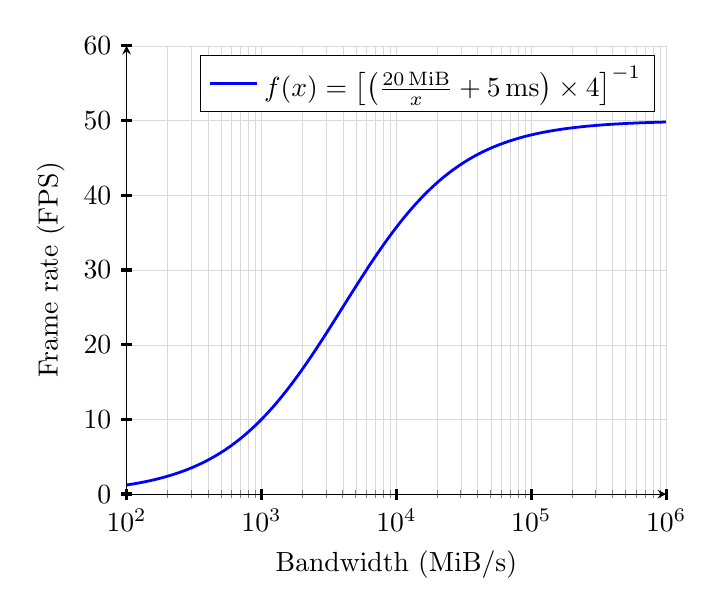
\begin{tikzpicture}
    \begin{semilogxaxis}[
        axis lines = left,
        xlabel = {Bandwidth (MiB/s)},
        ylabel = {Frame rate (FPS)},
        ymin = 0, ymax = 60,
        xmin = 100, xmax = 1000000,
        ytick distance=10,
        grid=both,
        grid style={line width=.1pt, draw=gray!30},
        every major tick/.append style={very thick, major tick length=4pt, black},
    ]
    
    \addplot [
        domain=1:1000000, 
        samples=1000, 
        color=blue,
        line width=1pt
    ]
    {1/((20/x + 0.005)*4)};
    
    \addlegendentry{$f(x) = \left[ \left( \frac{\SI{20}{MiB}}{x} + \SI{5}{ms} \right) \times 4 \right]^{-1}$}
    \end{semilogxaxis}
    \end{tikzpicture}

    \caption{Reachable frame rates with varying bandwidths for an example large model}
    \label{fig:large_model_bandwidth_analysis_example}
\end{figure}

\Cref{fig:large_model_bandwidth_analysis_example} shows that there is an horizontal asymptote at \SI{50}{FPS}\footnote{ $\lim_{x \to \infty} \left[ \left( \frac{\SI{20}{MiB}}{x} + \SI{5}{ms} \right) \times 4 \right]^{-1} = \SI{50}{Hz}$}.
Due to this, it is not possible to target an input frame rate of \SI{60}{FPS} for this model.
Even with an infinite write bandwidth, we can never reach \SI{60}{FPS}.
This limitation is due to the fixed processing latency of the four model parts (\SI{20}{ms}).
An input frame rate of \SI{30}{FPS} is possible and requires a write bandwidth of at least \SI{6}{GiB/s}.

With the bandwidth of the original \confignoc{} (\SI{763}{MiB/s}), we can target up to \SI{8}{FPS}\footnote{$\left[ \left( \frac{\SI{20}{MiB}}{\SI{763}{MiB/s}} + \SI{5}{ms} \right) \times 4 \right]^{-1} \approx \SI{8}{Hz}$}.
 
\section{Execution of the ResNet-101 model}
We will be looking at the execution of a large model on the \graicore{}.
In particular we will be using a specific model as an example throughout this subsection.

The ResNet-101 model is a deep neural network commonly used for computer vision applications \cite{heDeepResidualLearning2015}.
We will be using the ResNet-101 model from the \textit{Keras} library \cite{KerasDocumentationResNet} pretrained on the ImageNet database \cite{russakovskyImageNetLargeScale2014}
The ResNet-101 model has around \SI{44.5}{M} parameters in total.
An important feature of the ResNet architecture is the use of skip connections \cref{TODO}.

Due to the size (amount of parameters) of the ResNet-101 model, it is not possible to load the model on the \graicore{} at once.
This is still the case when representing the parameters with low-precision data types like 8-bit integers or floats (this also known as quantization).
Other solutions, such as model compression techniques exist to decrease the size of the model.
However, as explained earlier, this has its disadvantages such as decreased inference accuracy.

To allow the model to fit on the \graicore{} we will be looking at partitioning the model into smaller parts.
A model part is capable of being (completely) loaded on the \graicore{}.
By sequentially loading and processing each of the model parts, the full functionality of the original (large) model can be emulated.
The output data of each model part must be buffered outside the local memories, and will be used as input for the subsequent model part.
The amount of data to be buffered is dependent on the output shape of the final layer of a part.

% Due to ResNet's extensive use of skip connections, it is not straightforward to split/partition the model at any location. We therefore only consider locations in the network where it is easy to split. In most cases this is at locations right before or after a split connection.

\begin{figure}[hbtp]
    \centering
    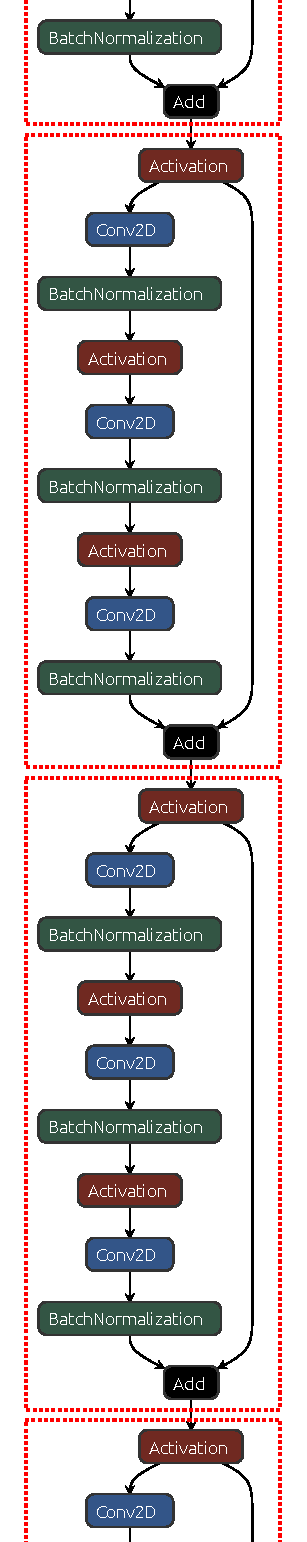
\includegraphics[angle=90, width=\linewidth]{assets/resnet101_residual_blocks.pdf}
    \caption{
    Snippet of a visualization of the ResNet-101 network.
    The red rectangles represent the residual blocks.
    }
    \label{fig:resnet101_residual_blocks}
\end{figure}

The ResNet architecture introduces so-called residual blocks (see \cref{fig:resnet101_residual_blocks}).
A residual block contains a collection of layers with a special type of connection from the beginning of the block until the end of the block.
This connection is also called a skip connection.
Due to these skip connections, it is not straightforward to split the ResNet-101 model at any location.
Splitting the model between two layers where also a skip connection resides, will introduce a few difficulties.
Firstly, you will require to buffer multiple outputs.
That is, the output data of the layer just before the split point and the output data of the skip connection.
Secondly, the two outputs need to be propagated to their respective destination layers.
These two outputs can have the same or different destination layer.
If they have different destinations, the output of the skip connection needs to be buffered until the network reaches a later stage.

In the context of the \graicore{}, this adds challenges to the system.
Not only does this increase the instantaneous total memory usage, it also increases the energy usage.
More energy is consumed due to the increased data to be buffered.
This is especially evident due to the need to buffer the data on some external memory.
Next to this buffering problem, software support must also be provided.
The current system only allows for a single input to the model. 

Due to these complexities, we keep the partitioning of the ResNet-101 model simple and only consider partitioning the network at locations where no skip connections appear.
Naturally, the main drawback of this is the reduces number of locations where partitioning can occur.

\begin{figure}[hbtp]
    \centering
    \subcaptionbox{MACs per residual block \label{fig:resnet101_macs}}[\textwidth]{
        \pgfplotstableread[col sep=semicolon]{assets/resnet101_stats.csv}\datatable
\begin{tikzpicture}
    \begin{axis}[
        width=\textwidth,    % set width
        height=0.3\textwidth, % and height
        ybar,
        enlarge x limits={rel=0.05},
        bar width=8pt,   % they were too wide
        xlabel={Residual block},
        ylabel={MACs},
        xlabel style={yshift=-1em},
        xtick=data,
        xticklabel style={rotate=45, font=\scriptsize, anchor=east},
        xticklabels from table={\datatable}{index},
    ]
    \addplot table[x expr=\coordindex, y={macs}]{\datatable};
    \end{axis}
\end{tikzpicture}

    }
    \subcaptionbox{Number of parameters per residual block \label{fig:resnet101_params}}[\textwidth]{
        \pgfplotstableread[col sep=semicolon]{assets/resnet101_stats.csv}\datatable
\begin{tikzpicture}
    \begin{axis}[
        width=\textwidth,    % set width
        height=0.3\textwidth, % and height
        ybar,
        enlarge x limits={rel=0.05},
        bar width=8pt,   % they were too wide
        xlabel={Residual block},
        ylabel={\# Parameters},
        xlabel style={yshift=-1em},
        xtick=data,
        xticklabel style={rotate=45, font=\scriptsize, anchor=east},
        xticklabels from table={\datatable}{index},
    ]
    \addplot table[x expr=\coordindex, y={params}]{\datatable};
    \end{axis}
\end{tikzpicture}
    }
    \caption{
        MACs and the number of parameters per residual block.
        The tuple $(x, y)$ represents the residual block at index $y$ of the stage at index $x$.
        \textit{Head} and \textit{tail} contain the remaining layers at the start and end of the network respectively.
    }
    \label{fig:resnet101_stats}
\end{figure}

The ResNet-101 model contains five so-called stages.
A stage is a collection of consecutive layers.
Only the first stage does not include any residual blocks.
The other stages contain different amounts of residual blocks as shown in \cref{fig:resnet101_stats}.

If we opt to split the network based on computational complexity, we look at the amount of multiply-accumulate (MAC) operations of the layers.
A MAC operation is essentially a multiplication operation followed by a addition operation.
Since we only perform splits between residual blocks, we combine the MACs of each layer in the residual blocks.
In \cref{fig:resnet101_macs}, we observe that the amount of MACs for each residual block is relatively similar.
We see small peaks at the start of each stage.
This is due to an additional convolution layer in the first residual block of a stage.
% A model or model part with more MACs generally is more heavy to run than those with less MACs (lower .
Generally, a model or model part with high number of MACs take longer to process fully.

In \cref{fig:resnet101_params}, we observe that the distribution of the parameters do vary significantly over the residual blocks.
The graph shows that the last few residual blocks carry a significant portion of the total parameters.
Again, we see small peaks at the start of each stage.
Naturally, a model part with a higher number of parameters will require more memory space.
Due to the uneven distribution of the parameters we have less flexibility with partitioning. 

\section{Splitting}
The ResNet-101 model has a total parameter count of around \SI{44.5}{M}.
Even if the parameters are quantized to an 8-bit datatype, the model will still not fit on the \graicore{} as a whole.
Weights stored on the \graicore{} require one extra bit.
% This extra bit is used as a mask that activates or deactivates the associated weight.
This extra bit is used to indicate whether a weight is removed (i.e., pruned) or not.
However, since we are using the original ResNet-101, no pruning has been applied to the weights.
We can roughly say that the network requires \SI{47.7}{MiB}\footnote{$\frac{\num{44496488} \times 9}{8} \times \frac{1}{2^{20}}$} of memory capacity for the parameters when quantized to 8 bits.
However, this does not include any mandatory header information and buffer space when mapping the network for the \graicore{}. 

The in-house compiler for the \graicore{} is complex and we will not get into detail.
In a nutshell, the compiler first optimizes the model by converting it to a so-called \textit{GrAI Model}.
Among other things, the optimized model slightly changes the architecture of the network and optionally performs post-training quantization \cref{TODO} for the weights.
The amount of MACs and parameters stay roughly the same.
Afterwards, it will map the layers of the model to the neuron cores.
The compiler can be instructed to optimize for inference latency.
This is done, for example, by mapping a single layer to multiple neuron cores to exploit parallelism.

Splitting the network between the residual blocks $(4, 18)$ and $(4, 19)$, we obtain two parts with roughly the same number of parameters (\SI{21.9}{M} and \SI{22.6}{M}).
For the weights, this is \SI{23.5}{MiB} and \SI{24.2}{MiB} respectively.

\hrulefill


\subsubsection{ResNet-101 partitioned in 5 parts}
One example partitioning is done as follows (note that the parameters are quantized to 8 bits).
The ResNet-101 model is partitioned in 5 parts.
The compiler is able to compile each of the parts, indicating that they are configurable on the \graicore{}.
The processing latency for each of the parts can be estimated by using the in-house \graipefruit{} simulator.
Furthermore, the compiler also provides us information about how much data must be written to each of the neuron cores.
Note that the compiler can map a layer to multiple neuron cores.
This requires the weights to be written to all neuron cores that require them.
This means that the \graicore{} contains duplicate weights.
The total data to write and processing latency for each part is shown in \cref{tab:resnet101_5parts}.

\begin{table}[hbtp]
\centering
\begin{tabular}{@{}llll@{}}
\toprule
\textbf{Part}  & \textbf{To write (MiB)} & \textbf{Latency (ms)} & \textbf{Time to configure (ms)} \\ \midrule
1              & 28.75                   & 7.08                  & 2.36                            \\
2              & 20.06                   & 2.65                  & 1.64                            \\
3              & 30.44                   & 4.01                  & 2.49                            \\
4              & 17.71                   & 2.34                  & 1.45                            \\
5              & 15.54                   & 2.04                  & 1.27                            \\ \midrule
\textbf{Total} & 112.51                  & 18.12                 & 9.22                            \\ \bottomrule
\end{tabular}
\caption{Statistics of the ResNet-101 model partitioned in 5 parts}
\label{tab:resnet101_5parts}
\end{table}
% Using the proposed \confignoc{}, we can reach a peak write bandwidth of 11.92 GB/s.
With the write bandwidth of the newly proposed \confignoc{} (\SI{11.92}{GiB/s}), we compute the time to configure each of the parts (see \cref{tab:resnet101_5parts}).
The sum of the configuration times and processing latencies is \SI{27.34}{ms}.
This means that we can (at best) process frames with an input frame rate of \SI{36.6}{FPS}\footnote{$\frac{1}{\SI{27.34}{ms}}$}.
% The compiler accepts many parameters that can affect the performance (e.g., inference latency or power usage) when the model is running on the \graicore{}.

% However, before mapping this network to the \graicore{}, the model needs to be converted to a new model optimized for the \graicore{} called GrAIModel. Among other things, the optimized model slightly changes the architecture of the network and performs quantization for the weights (if this was chosen). We observe that the MACs stay roughly the same while the number of parameters do change.

% When compiling the network/model for the \graicore{}, it firstly gets converted to a GrAIModel. Afterwards, it will map the layers to the neuron cores. For improving the inference latency, it can map (parts of) a single layer to multiple neuron cores to exploit parallelism.

% The compiler for the \graicore{} is complex and we will not get into detail. In a nutshell, the compiler optimizes the input model to a GrAIModel, afterwards it will map the layers to the neuron cores. It can optimize for inference latency by exploiting parallelism. This is done by, for example, mapping a single layer to multiple neuron cores.


%%%

% There are many ways to partition a model. 
% Amount of parts (there is a minimum)
% Distribution of parameters
% Distribution of FLOPS/MACs

% We use the in-house compiler to find a valid mapping for the \graicore{}, with focus on low processing latency. The compiler also outputs files necessary for simulating the networks with \graipefruit{}. \graipefruit{} is used to approximate the processing latency of a network.
% Note that the compiler is a complex piece of software. Since it accepts many parameters, it is difficult to find an optimal mapping. 

% This section discusses various modifications to the config NoC that can be implemented to improve the configuration speed of the GrAICore.

% TODO add introduction to chapter
\lipsum[1]
% % \section{Proposed \confignoc{} specifications}
\section{Proposed specifications}
\label{sec:proposed_noc}
% In this section, we provide a detailed specification of the proposed \confignoc{} and interface for \graicore{} based on the analysis and observations presented in the previous sections of this document.
To improve the bandwidth of configuration with the \confignoc{}, a set of changes is proposed. Firstly, we propose to widen the links from 16 bits to 64 bits.
This allows for phits of 64 bits in size.
This change provides us with a potential bandwidth increase of 4x.
An immediate increase to 64 bits instead of 32 bits is preferred as it allows for one-time change in the design and verification effort.
Another benefit is the synergy with the unified memories.
Since the SRAMs have 64-bit memory words and can write one memory word of 64 bits every cycle, there is no need to buffer multiple (smaller) phits before writing them to the SRAM.
This first change proposal provides a peak bandwidth of \SI{3}{GiB/s}.

Next, by dividing the \confignoc{} into two equally sized (virtual) zones with their own external interface, we can benefit from parallel configuration of two cores (one per zone) and therefore, another 2x increase in bandwidth.
These two changes provide a bandwidth of around \SI{6}{GiB/s}. 
The amount of zones and injection points can be expanded in the future at relatively small costs if necessary.

Lastly, the aforementioned changes require a change in the packet format.
The new packet format benefits from less overhead per chunk of payload data.
Since we opt for a link width of 64, the size of a single phit also increases to 64 bits.
All header information fits within a single phit of 64 bits.
The data phits following the header are fully utilized for payload data.
The format of the header is shown in \cref{fig:packet_format_header_new}.
With a length field of 6 bits, we can specify up to 65 data phits for a single packet.
This is a sufficient amount as argued in the previous section. 
Compared to the current packet format, an additional bandwidth increase of almost 2x can be gained with this new packet format.

\begin{figure}[hbtp]
    \centering
    \resizebox{\linewidth}{!}{
        \newcommand{\fakesixtyfourbits}[1]{%
    \ttfamily
    \small
    \ifnum#1=1234567890
        #1
    \else
        \ifnum#1=40
            % \count32=#1
            % \advance\count32 by 48
            % \the\count32%
            63%
        \else
            \ifnum#1<37
                #1%
            \else
                \ifnum#1=38
                    $\cdots$%
                \fi
            \fi
        \fi
    \fi
}

\begin{bytefield}[
    boxformatting={\centering\ttfamily},
    % bitformatting={\ttfamily\small},
    bitformatting={\fakesixtyfourbits},
    endianness=big,
    bitwidth=1.5em,
    bitheight=2.5em
]{41}
% \bitheader{0-45} \\
\bitheader{40, 38, 36, 30, 10, 6, 2, 0} \\

\bitbox{5}[bgcolor=lightgray]{Unused} &
\bitbox{6}[bgcolor=lightyellow]{Length[5:0]} &
\bitbox{20}[bgcolor=lightcyan]{Address[19:0]} &
\bitbox{4}[bgcolor=lightred]{Dest. Y} &
\bitbox{4}[bgcolor=lightorange]{Dest. X} &
\bitbox{2}[bgcolor=lightgreen]{\scriptsize Packet type} \\

\end{bytefield}
    }
    \caption{Proposed packet header format}
    \label{fig:packet_format_header_new}
\end{figure}

Through increasing the link width, adding an additional injection point, and adopting a new packet format, it’s possible to achieve a significant peak bandwidth improvement of nearly 16x.
Specifically, this translates to upgrading from an initial bandwidth of \SI{0.75}{GiB/s} to a substantial \SI{11.92}{GiB/s}.
Moreover, additional increase in bandwidth can be obtained by increasing the amount of injection points.

% To obtain an insight into the power consumption with the introduction of the config NoC changes in \cref{TODO} and model configuration using external memory we will provide an comprehensive analysis.
% To get an approximation of the power consumption when configuring the GrAICore with a model and processing frames with it, we will provide calculations with energy parameters acquired from internal sources.

When configuring the GrAICore and processing an input frame, the major components that consume energy are as follows:
\begin{itemize}
    \item Configuration
    \begin{itemize}
        \item Reading data from the external memory
        \item Transferring data from the external memory to the config NoC
        \item Phits traversing (i.e., hops) through the config NoC
        \item Writing data to the neuron core's SRAM
    \end{itemize}
    \item Processing
    \begin{itemize}
        \item Processing the input frame by the model
    \end{itemize}
\end{itemize}

% \section{Power analysis calculations}
The calculation for the total energy cost for configuring the GrAICore and processing an input frame will be explained next.

\subsection{Configuration}
The configuration energy consists of the reading, transferring and writing of data from the external memory to the GrAICore's SRAMs. 

Let $C$ be the set of tuples holding the coordinates of every core:
\begin{equation}
    C = \{\,\left(x,y\right) \in \mathbb{N}^2 \mid 1 \leq x \leq 12 \wedge 0 \leq y \leq 11 \,\} 
\end{equation}

% \Cref{fig:model_data_heapmap} shows the amount of data from an arbitrary model that needs to be written to each of the 144 neuron cores.
\Cref{fig:model_data_heapmap} shows for a 80\% pruned version of ResNet-50\footnote{Internally named \texttt{resnet50\_pruned80\_star}} the amount of data that needs to be written to each of the 144 neuron cores.
We observe that the data is not uniformly distributed across the SRAMs.
Therefore, we require information how much data needs to be transferred to each SRAM.

\begin{figure}[hbtp]
    \centering
    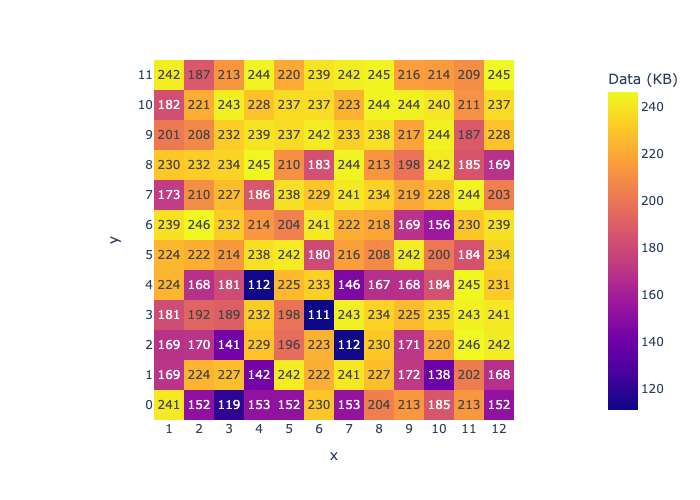
\includegraphics[width=0.8\linewidth]{assets/model_data_heatmap.png}
    \caption{Amount of data to be written to each core for the ResNet-50 model (80\% pruned).}
    \label{fig:model_data_heapmap}
\end{figure}

Let $D$ be a matrix of $12 \times 13$ with $D_{i,j}$ denoting the amount of bytes to be written to core $\left( i,j \right)$.
$D$ has an additional column due to the x-coordinates not starting from index $0$.
Its left-most column is unused (i.e., $D_{0,0}, D_{0,1}, \cdots, D_{0,11}$).
This matrix can be constructed from the artifacts outputted by the compiler.

The number of phits to be transferred through the config NoC influences the total energy costs.
In particular, the amount of phits to be transferred affects the number of hops to be taken in total and the amount of data to be written to the SRAMs.
Therefore, we need to determine how many phits needs to be transferred to each neuron core.
% The number of phits to be transferred influences the energy cost in the config NoC hops and SRAM writes.
% A packet can contain up to 520 bytes\footnote{$65 \times \frac{64}{8}$} of payload data. 
A packet can contain up to 65 data phits, that is $65 \times \SI{64}{b} = \SI{520}{B}$ of payload data.
% If we transfe
Suppose we need to transfer $d$ bytes to a neuron core, we then require a total of $\left\lfloor \frac{d}{520} \right\rfloor$ packets with 65 data phits.
% If $d \bmod 520 > 0$, then there is an additional packet consisting of $\left\lceil \frac{\left( d \bmod 520 \right) \times 8}{64}\right\rceil$ data phits.
If $\left( d \bmod 520 \right) > 0$, then there is an additional packet for the remaining $\left( d \bmod 520 \right)$ bytes of data.
The remaining packet will consist of $\left\lceil \frac{d \bmod 520}{8}\right\rceil$ data phits.
Note that each packet also contains a single phit of 64 bits for the header information.


The total energy cost for configuring the GrAICore can be estimated with the following equation:
\begin{equation}
    E_{\textrm{config}} = E_{\textrm{ext\_mem}} + E_{\textrm{noc}} + E_{\textrm{write}}
\end{equation}

With:
\begin{align*} 
E_{\textrm{ext\_mem}} &= 
        \sum_{c \in C}^{}{E_\textrm{read\_ext\_mem}(D_c) + E_{\textrm{send\_to\_noc}}(D_c)} \\
E_{\textrm{noc}} &=
    E_{\textrm{hop}} \times \sum_{c \in C}^{}{N_\textrm{hops}(c) \times p_{\textrm{total}}(D_c)} \\
E_{\textrm{write}} &=
    E_{\textrm{sram\_write\_64b}} \times \sum_{c \in C}^{}{p_{\textrm{data}}(D_c)}
\end{align*}

And:
\begin{align*} 
N_{\textrm{hops}}(x,y) &=
    \begin{cases} 
        x + y & \textrm{if } 0 \leq y \leq 5 \\
        x + y - 6 & \text{if } 6 \leq y \leq 11
    \end{cases}
\\
p_{\textrm{total}}(d) &=
    \left\lfloor \frac{d}{520} \right\rfloor \times (65 + 1) + \left\lceil \frac{d \bmod 520}{8} \right\rceil + 1 =
    \left\lceil \frac{d}{8} \right\rceil + \left\lfloor \frac{d}{520} \right\rfloor + 1 
\\
p_{\textrm{data}}(d) &=
    \left\lfloor \frac{d}{520} \right\rfloor \times 65 + \left\lceil \frac{d \bmod 520}{8} \right\rceil =
    \left\lceil \frac{d}{8} \right\rceil
\end{align*}

\begin{eqexpl}[15mm]
    \item{$p_{\textrm{total}}(D_c)$} total phits (includes headers) for transferring $D_c$ bytes
    \item{$p_{\textrm{data}}(D_c)$} total data phits (excludes headers) for transferring $D_c$ bytes
    \item{$N_{\textrm{hops}}(c)$} the amount of hops required to reach a neuron core at coordinate $c$, starting from the router closest to the injection point. It has two sub-functions due to the new config NoC's dual injector architecture
    \item{$E_{\textrm{read\_ext\_mem}}(D_c)$} energy for reading $D_c$ bytes from the external memory
    \item{$E_{\textrm{send\_to\_noc}}(D_c)$} energy for sending $D_c$ bytes from the external memory to the config NoC
    \item{$E_{\textrm{hop}}$} energy for performing a single hop in the config NoC
    \item{$E_{\textrm{sram\_write\_64b}}$} energy for writing back 64 bits to a neuron core's SRAM
\end{eqexpl}

\subsection{Processing}
The frame processing energy is the energy consumed when the GrAICore processes a single frame with a configured model.
The energy for processing a single input frame is approximated as follows:
\begin{equation}
    E_{\textrm{frame}} = \textrm{avg\_util} \times \textrm{cores\_used} \times \textrm{processing\_latency} \times \SI{21}{mW}
\end{equation}

These parameters can all be extracted from GrAIPEFRUIT simulation results.
% % \section{Introduction}
Suppose we have a large model that does not fit on the GrAICore at once.
We will look at two strategies to partition the model to allow it to be executed on the GrAICore.

Assume we have a model of that requires \SI{60}{MiB} to be written to the GrAICore.
We are able to partition this model in two parts of \SI{30}{MiB} and four parts of \SI{15}{MiB}.
Furthermore, assume the latencies for processing and configuring as shown in \cref{tab:partitiong_strategies_example}.

\begin{table}[hbtp]
\centering
\begin{tabular}{@{}lll@{}}
\toprule
\textbf{Part} & \textbf{Processing (ms)} & \textbf{Configuration (ms)} \\ \midrule
\SI{30}{MiB}  & 4                        & 8                           \\
\SI{15}{MiB}  & 2                        & 4                          
\end{tabular}
\caption{TODO}
\label{tab:partitiong_strategies_example}
\end{table}

\section{Sequential configuration}
With the model partitioned in two parts of \SI{30}{MiB}, we can only fit one part on the GrAICore at a time.
Because of this, we can only configure and process in a sequential manner.
The configure and process timeline is illustrated in \cref{fig:schedule_sequential_configuration}.
% In total, to fully process the model in two parts, it takes \SI{16}{ms}.
The inference latency of a single input frame is \SI{16}{ms}.
\Cref{fig:schedule_sequential_configuration_extended} shows a timeline when processing multiple input frames in sequence, we see that we can reach a stable input frame rate of \SI{41.7}{FPS} ($\frac{1}{\SI{24}{ms}}$).

\begin{figure}[hbtp]
    \centering
    \resizebox{0.6\linewidth}{!}{
        \begin{RTGrid}[
    width=10cm,
    nosymbols=1,
]{2}{26}
    \RowLabel{1}{Configure}
    \RowLabel{2}{Process}

    \TaskExecution[execlabel=$p_1$,color=lightgray]{1}{0}{8}
    \TaskExecution[execlabel=$p_2$,color=lightgray]{1}{12}{20}

    \TaskExecution[execlabel=$p_1$,color=lightgray]{2}{8}{12}
    \TaskExecution[execlabel=$p_2$,color=lightgray]{2}{20}{24}
\end{RTGrid}
    }
    \caption{Example timeline of sequential configuration and processing}
    \label{fig:schedule_sequential_configuration}
\end{figure}

\begin{figure}[hbtp]
    \centering
    \resizebox{1.0\linewidth}{!}{
        \begin{RTGrid}[
    width=20cm,
    nosymbols=1,
]{2}{52}
    \RowLabel{1}{Configure}
    \RowLabel{2}{Process}

    \TaskExecution[execlabel=$p_1$,color=lightred]{1}{0}{8}
    \TaskExecution[execlabel=$p_2$,color=lightred]{1}{12}{20}

    \TaskExecution[execlabel=$p_1$,color=lightred]{2}{8}{12}
    \TaskExecution[execlabel=$p_2$,color=lightred]{2}{20}{24}

    \TaskExecution[execlabel=$p_1$,color=lightcyan]{1}{24}{32}
    \TaskExecution[execlabel=$p_2$,color=lightcyan]{1}{36}{44}

    \TaskExecution[execlabel=$p_1$,color=lightcyan]{2}{32}{36}
    \TaskExecution[execlabel=$p_2$,color=lightcyan]{2}{44}{48}

    \TaskRespTime{2}{0}{8}
    \TaskRespTime{2}{24}{8}
    
    % \TaskArrival{2}{8}
    \TaskDeadline{2}{24}
    % \TaskArrival{2}{32}
    \TaskDeadline{2}{48}
\end{RTGrid}
    }
    \caption{
    Example timeline of sequential configuration and processing for two input frames.
    The shaded areas represent periods where we expect an input frame.
    The arrows pointing down represent the points of time where the associated input frame has been fully processed.
    }
    \label{fig:schedule_sequential_configuration_extended}
\end{figure}

\section{Parallel configuration}
With the model partitioned in four parts, two parts of \SI{15}{MiB} can fit on the GrAICore at the same time.
This allows for a pipeline of configuration and processing.
For this approach to work, the neuron cores must be divided into two isolated segments/zones.
% With each zone able to contain a part.
Each of the zones will contain a single part.
With the introduction of the additional injection point, two model parts can be written to the local memories of the neuron cores in parallel.

\begin{figure}[hbtp]
    \centering
    \resizebox{0.65\linewidth}{!}{
        \begin{RTGrid}[
    width=10cm,
    nosymbols=1,
]{4}{26}
    \RowLabel{1}{Configure $Z_1$}
    \RowLabel{2}{Configure $Z_2$}
    \RowLabel{3}{Process $Z_1$}
    \RowLabel{4}{Process $Z_2$}

    \TaskExecution[execlabel=$p_1$,color=lightgray]{1}{0}{4}
    \TaskExecution[execlabel=$p_3$,color=lightgray]{1}{6}{10}

    \TaskExecution[execlabel=$p_2$,color=lightgray]{2}{0}{4}
    \TaskExecution[execlabel=$p_4$,color=lightgray]{2}{8}{12}

    \TaskExecution[execlabel=$p_1$,color=lightgray]{3}{4}{6}
    \TaskExecution[execlabel=$p_3$,color=lightgray]{3}{10}{12}

    \TaskExecution[execlabel=$p_2$,color=lightgray]{4}{6}{8}
    \TaskExecution[execlabel=$p_4$,color=lightgray]{4}{12}{14}
\end{RTGrid}
    }
    \caption{Example timeline of parallel configuration and processing}
    \label{fig:schedule_parallel_configuration}
\end{figure}

% This approach allows configuration of the two ``zones'' to be performed in parallel (see \cref{fig:schedule_parallel_configuration}).
% Also, processing and configuration can happen in parallel.
\Cref{fig:schedule_parallel_configuration} shows a timeline of a pipelined configuration and processing.
With this approach, the a constraint is that while the system is processing part $p_n$, the system should not reconfigure the zone where part $p_n$ resides at the same time.
$Z_1$ and $Z_2$ indicate one of the two independent zones.
Note that processing cannot be performed in parallel due to the input of the next part being dependent on the previous part's output.
% The following figure shows the timeline using ASAP scheduling for the tasks.
Observe that the configuration of $p_2$ can start \SI{2}{ms} later without affecting the total inference latency.
The total inference latency of this approach is \SI{10}{ms}.
This is a speedup of $1.6\times$ compared to the sequential configuration approach.
% with \SI{100}{FPS} ($\frac{1}{\SI{10}{ms}}$) as the highest manageable input frame rate.
% However, this does not allow for an input frame rate of \SI{100}{FPS} ($\frac{1}{\SI{10}{ms}}$).

\Cref{fig:schedule_parallel_configuration_extended} shows a possible timeline for three consecutive input frames at the highest manageable frame rate.
An arrow pointing up shows the arrival of an input frame.
It is apparent that the highest manageable frame rate is \SI{83.3}{FPS} ($\frac{1}{\SI{12}{ms}}$).

\begin{figure}[hbtp]
    \centering
    \resizebox{0.8\linewidth}{!}{
        \begin{RTGrid}[
    width=15cm,
    nosymbols=1,
]{4}{38}
    \RowLabel{1}{Configure $Z_1$}
    \RowLabel{2}{Configure $Z_2$}
    \RowLabel{3}{Process $Z_1$}
    \RowLabel{4}{Process $Z_2$}

    \TaskExecution[execlabel=$p_1$, color=lightred]{1}{0}{4}
    \TaskExecution[execlabel=$p_3$, color=lightred]{1}{6}{10}

    \TaskExecution[execlabel=$p_2$, color=lightred]{2}{0}{4}
    \TaskExecution[execlabel=$p_4$, color=lightred]{2}{8}{12}

    \TaskExecution[execlabel=$p_1$, color=lightred]{3}{4}{6}
    \TaskExecution[execlabel=$p_3$, color=lightred]{3}{10}{12}

    \TaskExecution[execlabel=$p_2$, color=lightred]{4}{6}{8}
    \TaskExecution[execlabel=$p_4$, color=lightred]{4}{12}{14}
    %%%
    \TaskExecution[execlabel=$p_1$, color=lightcyan]{1}{12}{16}
    \TaskExecution[execlabel=$p_2$, color=lightcyan]{2}{14}{18}

    \TaskExecution[execlabel=$p_1$, color=lightcyan]{3}{16}{18}
    \TaskExecution[execlabel=$p_2$, color=lightcyan]{4}{18}{20}

    \TaskExecution[execlabel=$p_3$, color=lightcyan]{1}{18}{22}
    \TaskExecution[execlabel=$p_4$, color=lightcyan]{2}{20}{24}

    \TaskExecution[execlabel=$p_3$, color=lightcyan]{3}{22}{24}
    \TaskExecution[execlabel=$p_4$, color=lightcyan]{4}{24}{26}
    %%%
    \TaskExecution[execlabel=$p_1$, color=lightgreen]{1}{24}{28}
    \TaskExecution[execlabel=$p_2$, color=lightgreen]{2}{26}{30}

    \TaskExecution[execlabel=$p_1$, color=lightgreen]{3}{28}{30}
    \TaskExecution[execlabel=$p_2$, color=lightgreen]{4}{30}{32}

    \TaskExecution[execlabel=$p_3$, color=lightgreen]{1}{30}{34}
    \TaskExecution[execlabel=$p_4$, color=lightgreen]{2}{32}{36}

    \TaskExecution[execlabel=$p_3$, color=lightgreen]{3}{34}{36}
    \TaskExecution[execlabel=$p_4$, color=lightgreen]{4}{36}{38}
    %%%
    % \TaskArrival{3}{4}
    % \TaskArrival{3}{16}
    % \TaskArrival{3}{28}
    
    \TaskRespTime{3}{0}{4}
    \TaskRespTime{3}{14}{2}
    \TaskRespTime{3}{26}{2}
    
    \TaskDeadline{4}{14}
    \TaskDeadline{4}{26}
    \TaskDeadline{4}{38}
\end{RTGrid}

    }
    \caption{
    Example timeline of parallel configuration and processing for three input frames.
    The shaded areas represent periods where we expect an input frame.
    The arrows pointing down represent the points of time where the associated input frame has been fully processed.
    }
    \label{fig:schedule_parallel_configuration_extended}
\end{figure}



\newpage
\printbibliography[heading=bibintoc]

\end{document}
